%!TEX TS-program = pdflatex
%!TEX root = tesi.tex
%!TEX encoding = UTF-8 Unicode

\chapter{Il Dataset}

Innanzitutto si specifica che con la parola Scarto si indica l'immagine di una carcassa che presenta colla sul fondo, pezzo che quindi dovrà essere scartato.
Invece con la parola Conforme si indica l'immagine di una carcassa nella quale la colla è stata depositata correttamente, quindi con fondo pulito.

In questo capitolo verranno descritti il \textit{dataset}, le problematiche più importanti delle immagini e gli algoritmi principali con cui sono state manipolate.
Il capitolo si chiude con la tecnica del \textit{data augmentation}.

\section{Problematiche Principali}

\subsection{Dataset Piccolo e Sbilanciato}
La prima difficoltà insorge ancora prima di ispezionare le immagini del \textit{dataset}.
Infatti questo non solo comprende solamente 1749 immagini, ma è anche fortemente sbilanciato:
\begin{itemize}
    \item 1719 immagini sono Conformi;
    \item 30 immagini sono Scarti.
\end{itemize}
A questo punto è corretto chiedersi se le quasi duemila immagini del \textit{dataset} siano sufficienti ai nostri scopi.
Nel campo del \textit{Machine Learning}, ed ancora di più in quello del \textit{Deep Learning}, non è raro che il numero di elementi in un \textit{dataset} sia dell'ordine delle decine di migliaia se non di quello delle centinaia di migliaia.
Basti pensare ai \textit{dataset} più famosi ed usati:
\begin{itemize}
  \item MNIST~\cite{mnist} è un \textit{dataset} molto famoso contenente $70000$ cifre disegnate a mano appartenenti a $10$ classi in totale.
    È allo stesso tempo sia il punto di partenza dei principianti, perché di facile manipolazione, sia il campo di prova degli esperti, sul quale vengono allenati nuovi modelli prima di testarli su compiti più complessi.

  \item CIFAR-10~\cite{cifar} contiene $60000$ immagini a colori suddivise in 10 classi da 6000 immagini l'una.
    Le classi comprendono alcuni tipi di veicoli ed animali.
    Date le dimensioni ridotte delle immagini, appena $32$x$32$ pixel, il \textit{dataset} occupa meno di $200 MB$, questo permette di allenare reti neurali in tempi ragionevoli.

 \item ImageNet~\cite{imagenet} con i suoi 14 milioni di immagini è il più grande \textit{dataset} che sia mai stato creato.
    I più grandi esperti nel campo del \textit{Machine Learning} si sfidano annualmente su questo \textit{dataset}.
    Contiene decine di migliaia di classi e le sue immagini sono in gran parte fotografie scattate da volontari, che quindi hanno condizioni di luminosità e colori molti diversi tra loro.
    Possono variare anche la dimensione e l'orientamento, orizzontale o verticale, delle immagini.

\end{itemize}

Ciascuno di questi \textit{dataset} è stato etichettato\footnote{in inglese \textit{labeled} da \textit{label}, etichetta} a mano.
Ciò significa che ad ogni immagine è stata assegnata, a mano, una classe di appartenenza.
Prendendo in esempio MNIST, se un'immagine raffigura la cifra $7$ allora sarà etichettata con il \textit{label seven} ed apparterrà alla classe di immagini in cui compare la cifra $7$.
Allo stesso modo le immagini di ImageNet hanno etichette come \textit{dog}, \textit{cat}, \textit{bird}, \textit{car}, \textit{bike}, ecc\dots %TODO forma corretta??
%Il nostro contiene due classi: Conforme e Scarto.

Sembrerebbe che possedere 2000 immagini appena renda impossibile applicare algoritmi di \textit{Machine Learning}.
In realtà osservando i Conformi, in figura~\ref{fig:esempi_conformi} sono stati riportati alcuni esemplari significativi, ci si accorge che i pezzi sono molto simili.
Questo non ci sorprende, dato che i pezzi vengono generati meccanicamente, è perfettamente lecito supporre che nessuna carcassa abbia delle caratteristiche completamente differenti dalle altre.
Le principali diversità sono dovute ad imperfezioni superficiali come graffi o macchie.
Si può quindi dire che la distribuzione dei pezzi conformi è descritta bene anche da un numero limitato di esemplari.
Purtroppo il sistema di acquisizione immagini introduce ulteriori fattori di diversità come la posizione delle balze e la luminosità, ma questi fattori potranno essere gestiti senza troppe difficoltà.
Concludiamo che il numero di Conformi a nostra disposizione è sufficiente ai nostri scopi.

\begin{figure}[ht] % TODO
  \begin{center}
    \begin{tabular}{ccc}

  \begin{subfigure}{.3\linewidth}
    \centering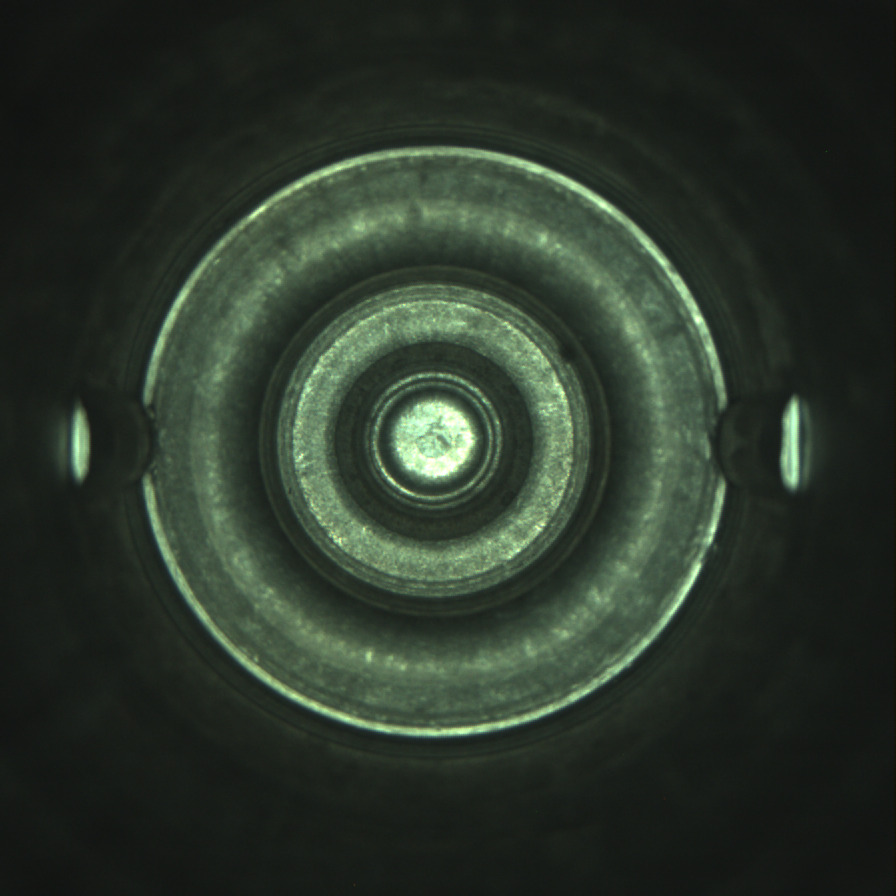
\includegraphics[width=\textwidth]{128___16760_0_0_1_OnLineAnalysis}
    \caption{}
  \end{subfigure} &

  \begin{subfigure}{.3\linewidth}
      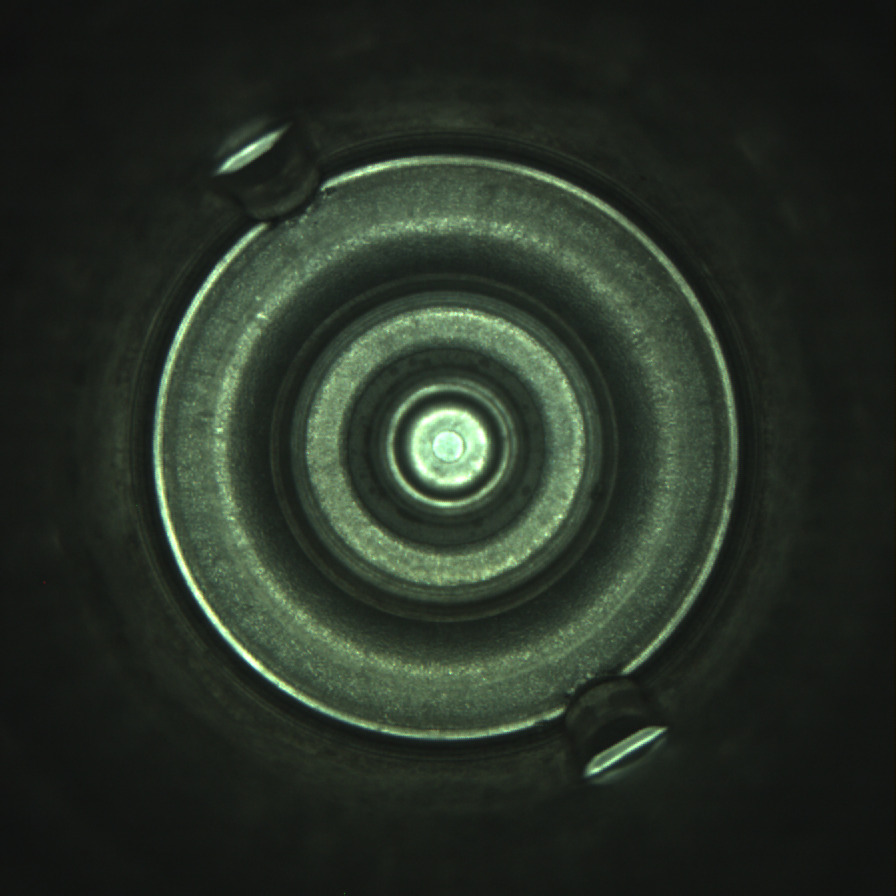
\includegraphics[width=\textwidth]{128___17986_1_1_1_OnLineAnalysis}
      \caption{}
    \end{subfigure} &

  \begin{subfigure}{.3\linewidth}
      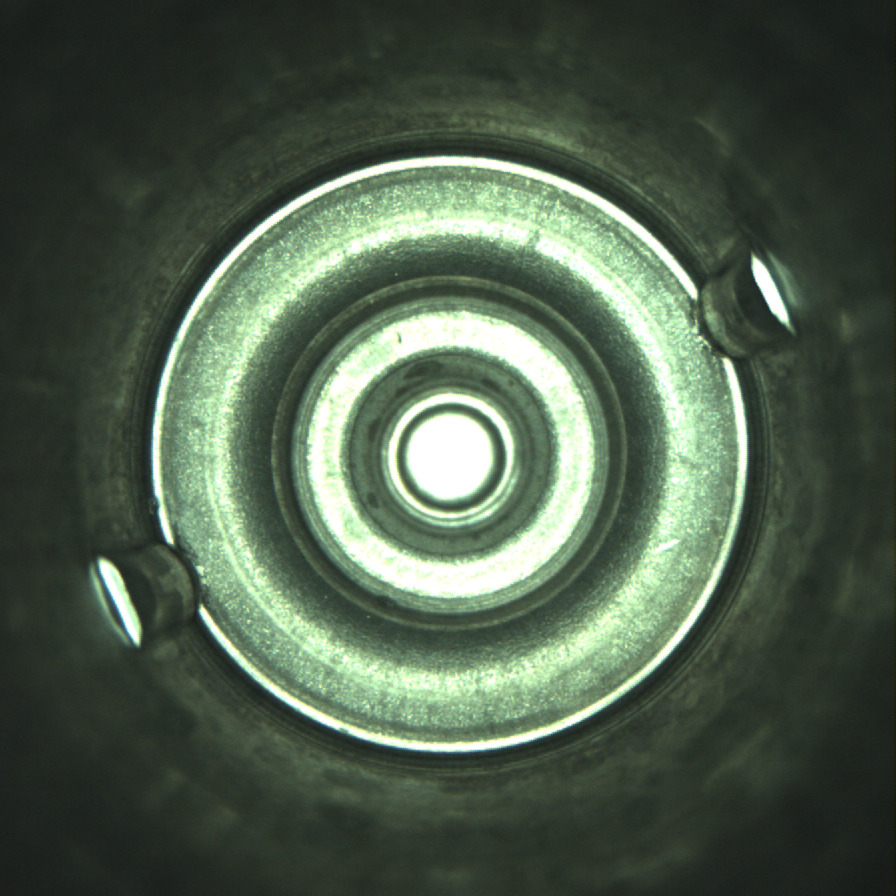
\includegraphics[width=\textwidth]{128___18037_1_0_1_OnLineAnalysis}
      \caption{}
    \end{subfigure} \\ \\

  \begin{subfigure}{.3\linewidth}
      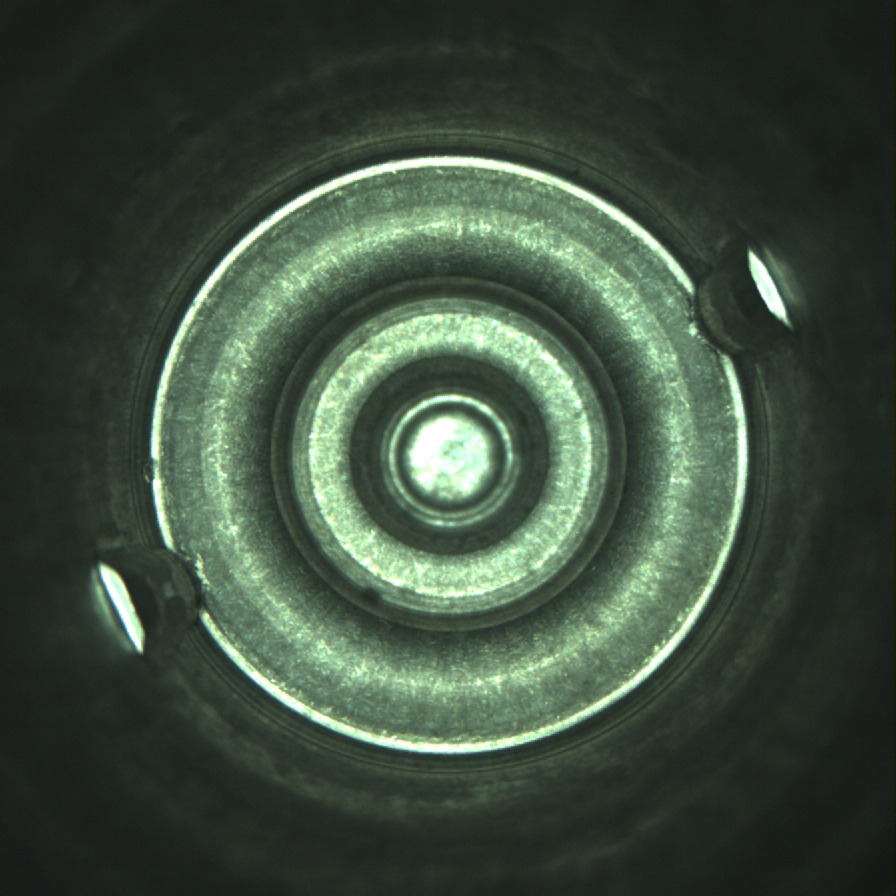
\includegraphics[width=\textwidth]{128___289_1_0_1_OnLineAnalysis}
      \caption{}
    \end{subfigure} &

  \begin{subfigure}{.3\linewidth}
      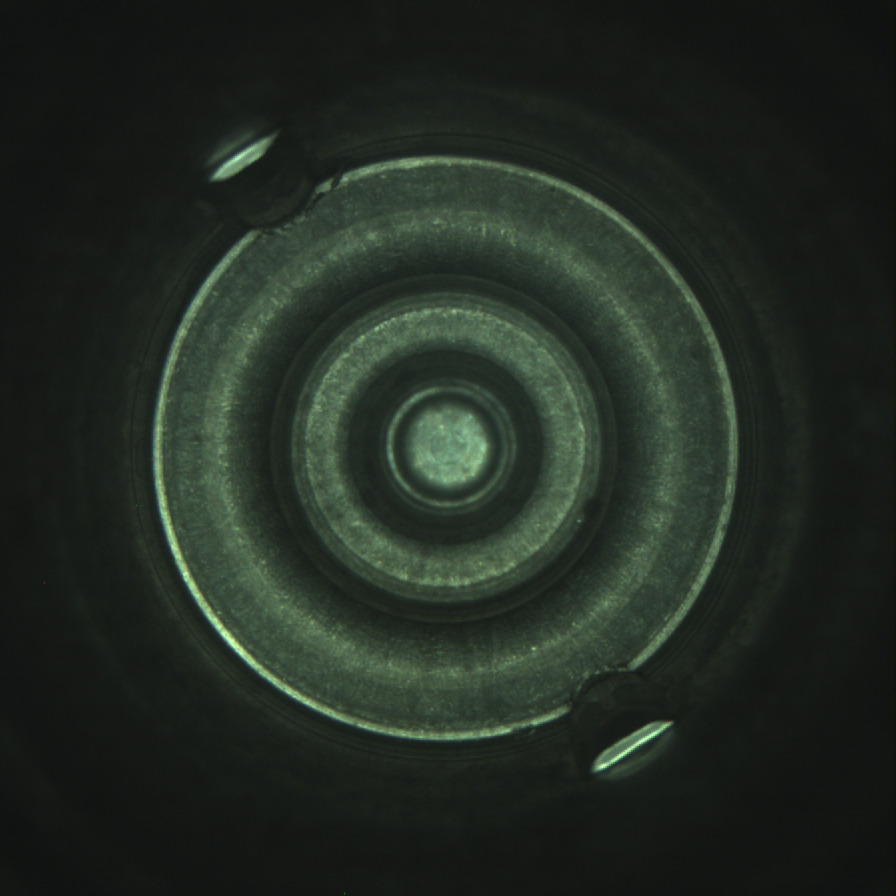
\includegraphics[width=\textwidth]{128___290_1_1_1_OnLineAnalysis}
      \caption{}
    \end{subfigure} &

    \begin{subfigure}{.3\linewidth}
      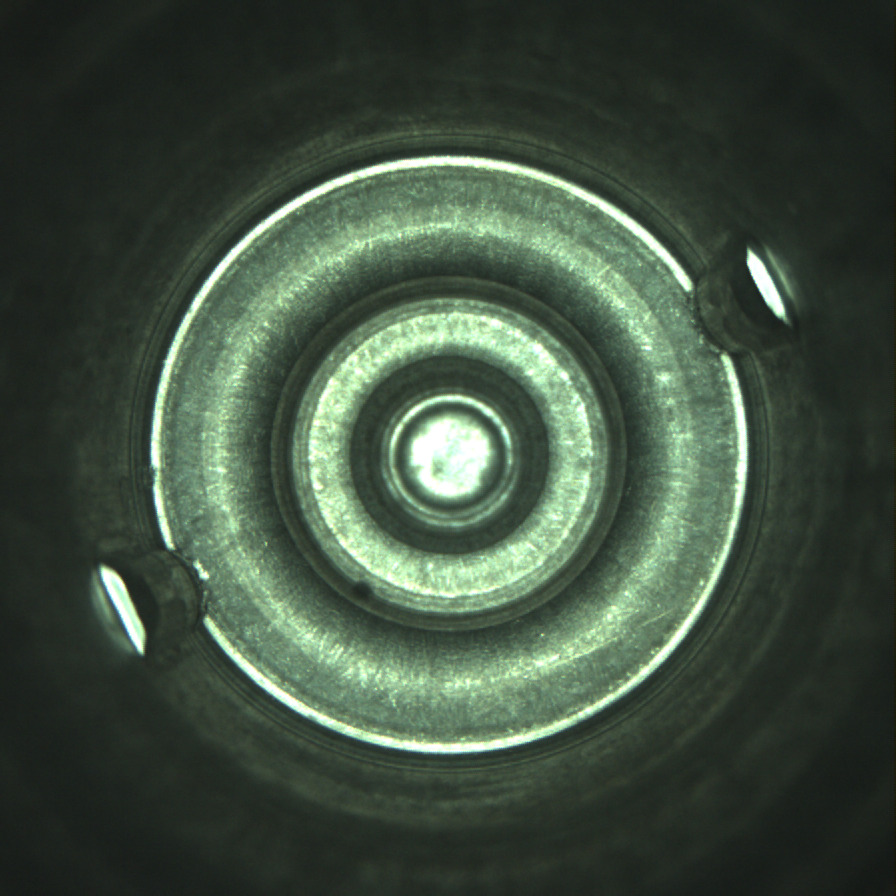
\includegraphics[width=\textwidth]{128___297_1_0_1_OnLineAnalysis}
      \caption{}
    \end{subfigure} \\

    \end{tabular}
    \caption{Alcune carcasse Conformi}
    \label{fig:esempi_conformi}
  \end{center}
\end{figure}

% https://tex.stackexchange.com/questions/333249/controlling-subfigure-captions-and-subfigure-placement

Non possiamo dire lo stesso per gli Scarti.
Se già la statistica ci lascia sospettare che $30$ esemplari non possono ritenersi significativi, allora questo sospetto diventa certezza quando si analizzano le caratteristiche della colla nelle immagini Scarto.  
Come si vede in figura~\ref{fig:esempi_scarti} la colla può presentarsi in forma di gocce più o meno circolari oppure come sbaffi di grossezza e lunghezza variabili.
Anche la quantità di superficie coperta dalla colla può variare notevolmente, passando da aree ridotte e localizzate ad aree estese e di conformazioni singolari.
Infine notiamo che la posizione del rimasuglio di colla all'interno della carcassa non è in relazione con la posizione delle balze e che la presenza dei gradini sul fondo non la obbliga in alcun modo a scivolare fino al centro.

\begin{figure}[ht] % TODO
  \begin{center}
    \begin{tabular}{ccc}

  \begin{subfigure}{.3\linewidth}
    \centering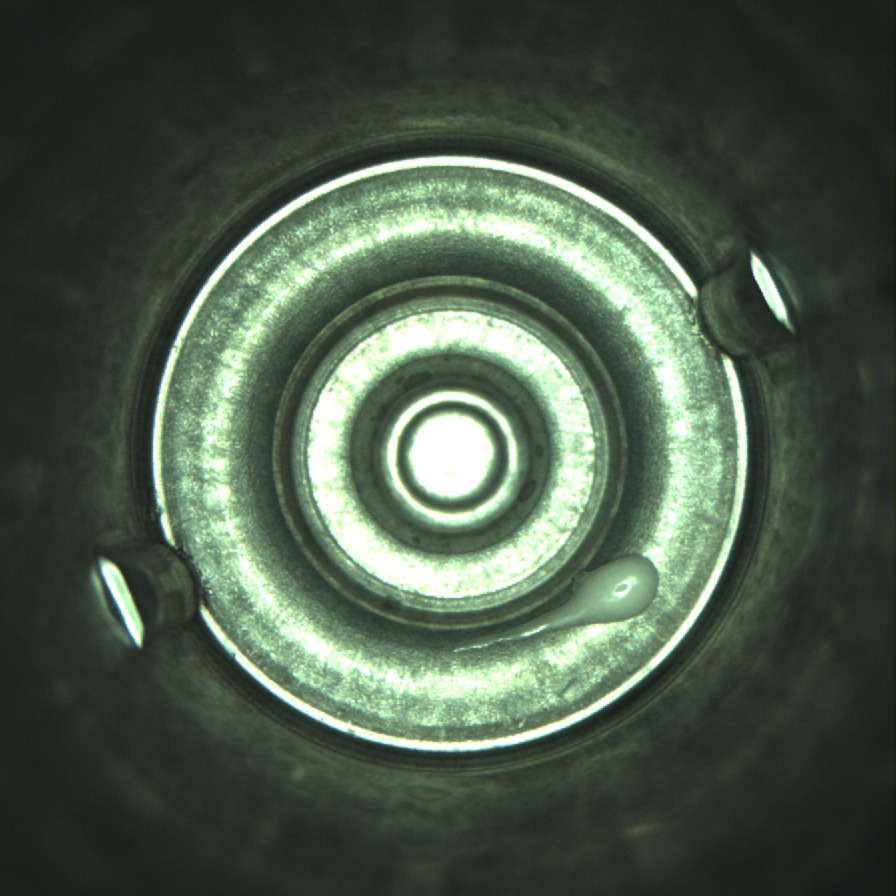
\includegraphics[width=\textwidth]{128___14097_1_0_1_OnLineAnalysis}
    \caption{}
  \end{subfigure} &

  \begin{subfigure}{.3\linewidth}
      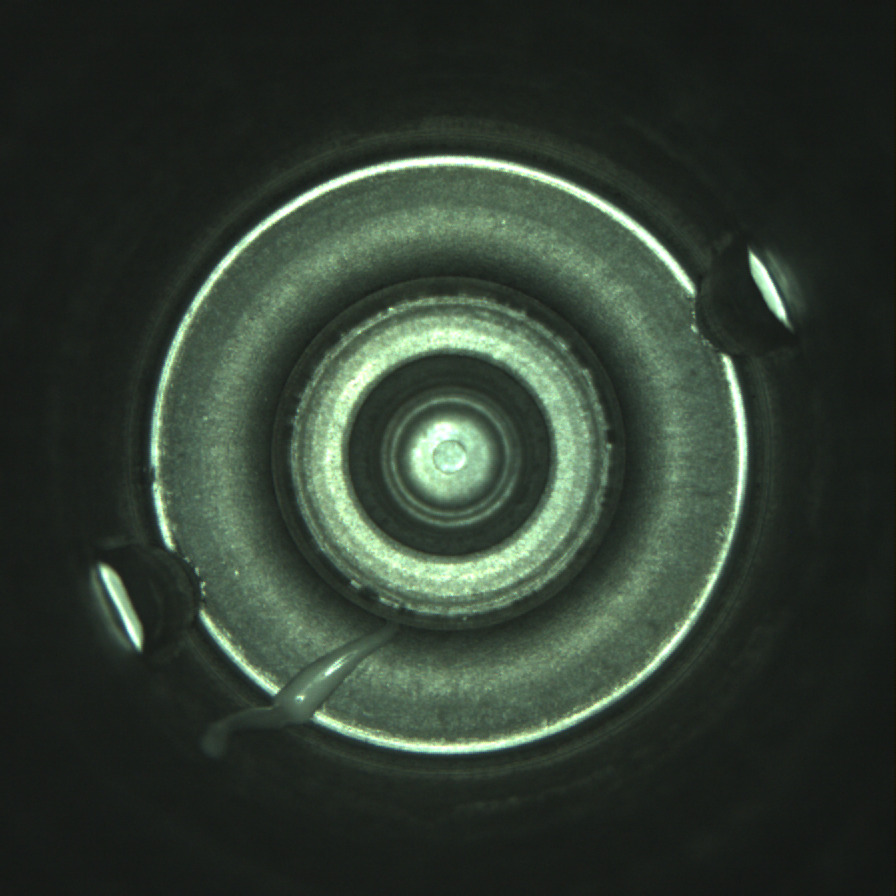
\includegraphics[width=\textwidth]{128___14177_1_0_1_OnLineAnalysis}
      \caption{}
      \label{fig:esempi_scarti_sbaffo}
    \end{subfigure} &

  \begin{subfigure}{.3\linewidth}
      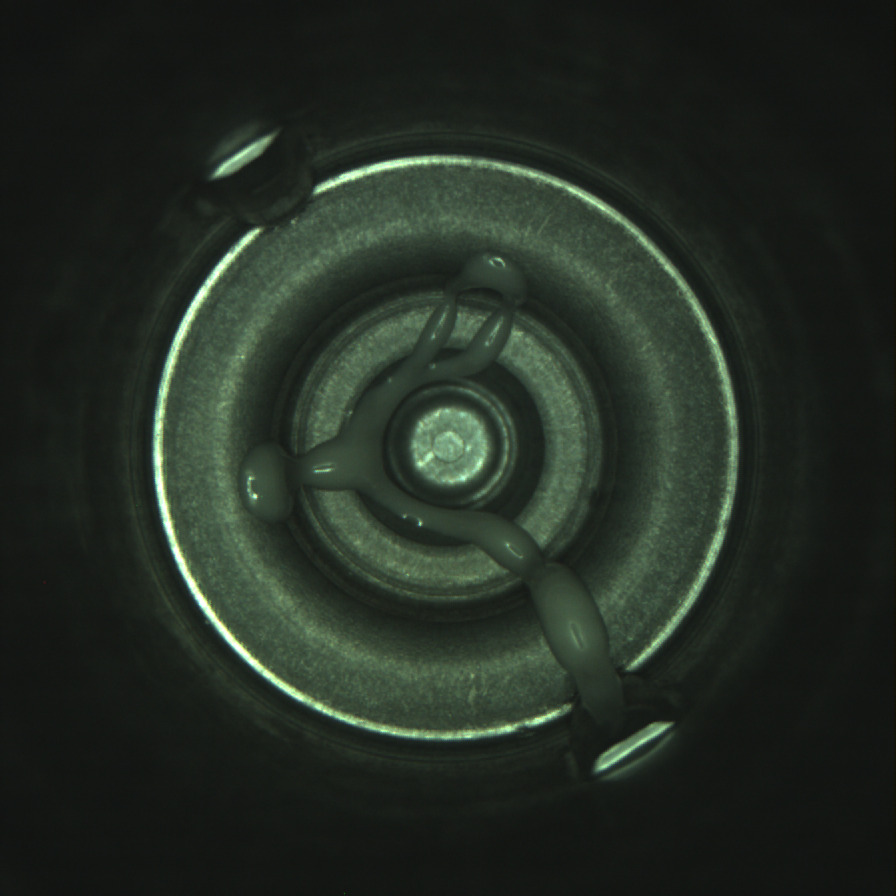
\includegraphics[width=\textwidth]{128___22886_1_1_1_OnLineAnalysis}
      \caption{}
    \end{subfigure} \\ \\

  \begin{subfigure}{.3\linewidth}
      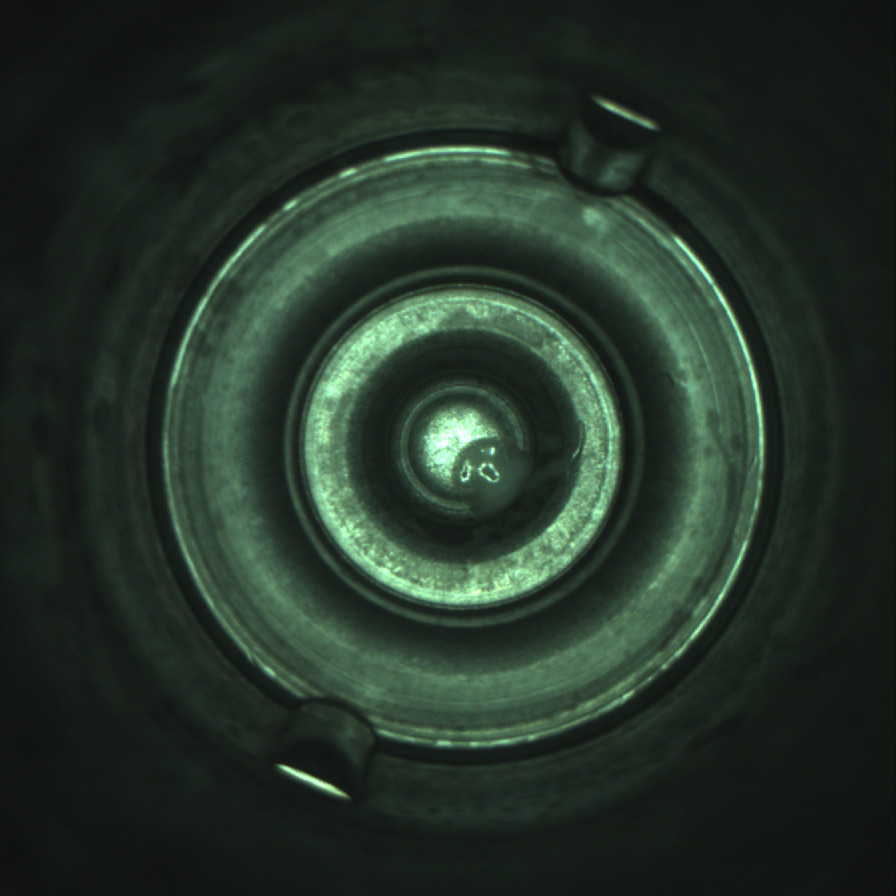
\includegraphics[width=\textwidth]{128___33657_0_0_1_OnLineAnalysis}
      \caption{}
      \label{fig:esempi_scarti_goccia}
    \end{subfigure} &

  \begin{subfigure}{.3\linewidth}
      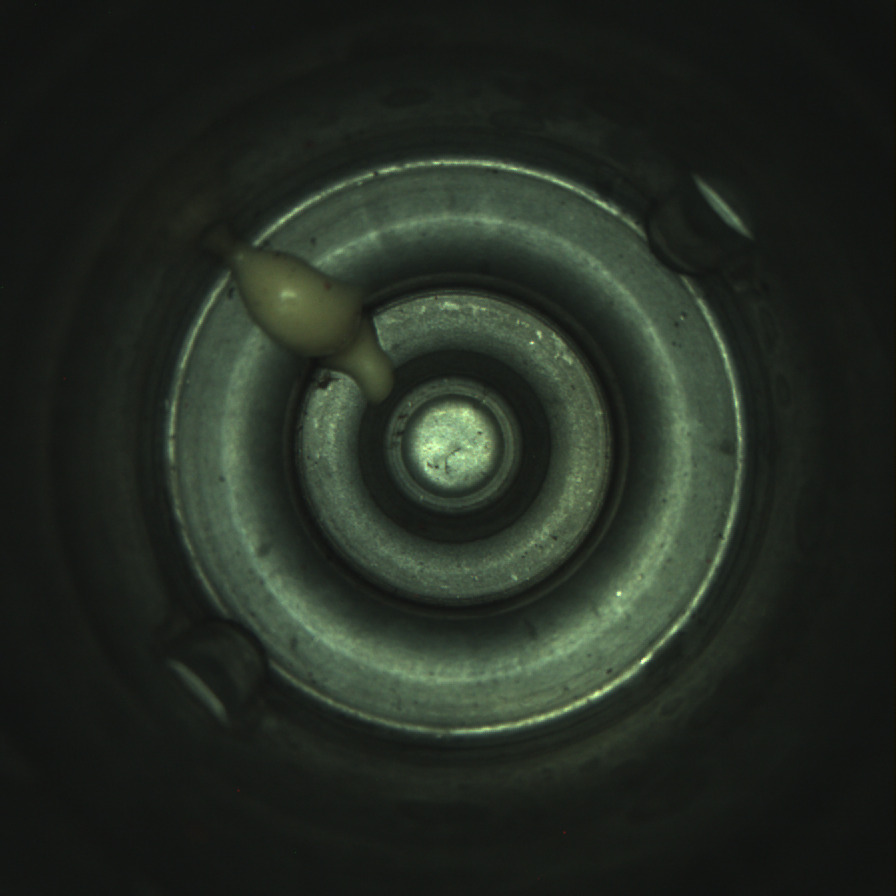
\includegraphics[width=\textwidth]{128___35_0_1_1_OnLineAnalysis}
      \caption{}
    \end{subfigure} &

    \begin{subfigure}{.3\linewidth}
      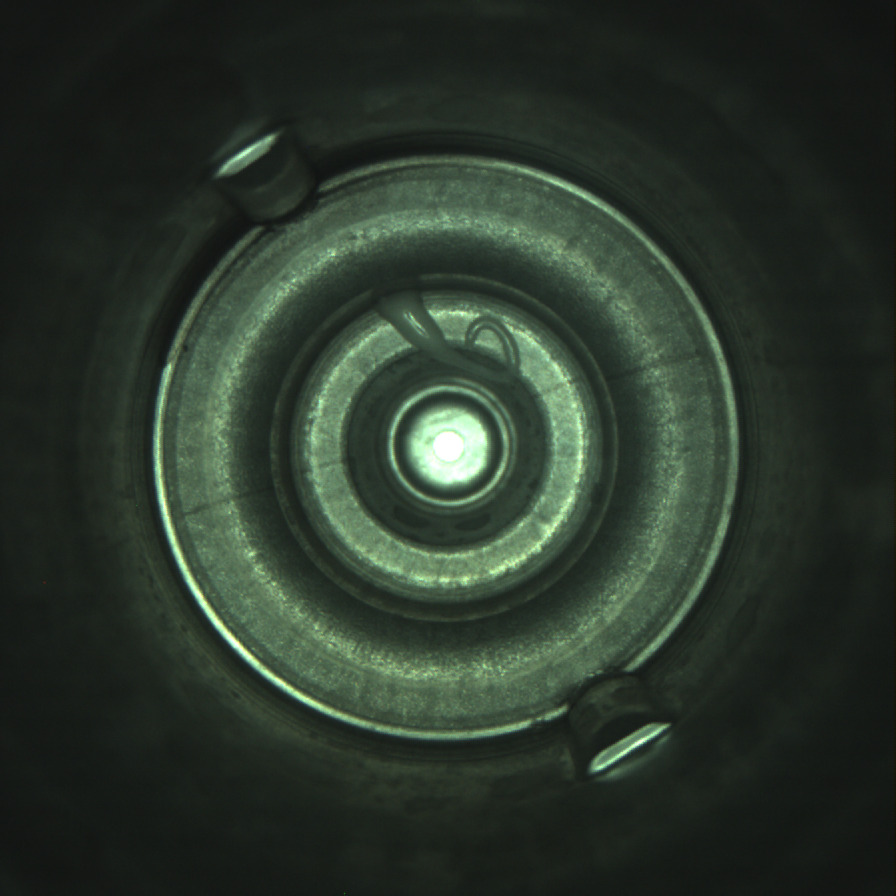
\includegraphics[width=\textwidth]{128___5668_1_1_1_OnLineAnalysis}
      \caption{}
    \end{subfigure} \\

    \end{tabular}
    \caption{Alcune carcasse Scarto}
    \label{fig:esempi_scarti}
  \end{center}
\end{figure}

Per analizzare meglio le modalità con cui potrebbe essere generato uno Scarto si supponga che il macchinario abbia commesso un errore: dall'ugello è uscita un certa quantità di colla in esubero.
A seconda della posizione dell'ugello rispetto alla carcassa si può immaginare che la colla raggiunga il fondo in vari modi, proviamo ora ad illustrarne due:
\begin{itemize}
  \item nel primo caso si immagina che il braccio abbia già depositato l'anello di colla e che si stia allontanando dalla carcassa.
    La colla in esubero cadrebbe sotto forma di goccia fino a raggiungere il fondo del pezzo.
    Questo potrebbe esse il caso per la figura~\ref{fig:esempi_scarti_goccia};
  \item nel secondo caso si ipotizza che la colla in esubero faccia parte dell'anello appena depositato e che, a causa delle vibrazioni o di altri fattori simili, coli raggiungendo il fondo della carcassa.
    Questo potrebbe esse il caso per la figura~\ref{fig:esempi_scarti_sbaffo}.
\end{itemize}

Data la grande varietà di modi in cui la colla può presentarsi, concludiamo che gli esemplari forniti per la classe Scarto la descrivono soltanto in modo parziale.
Ciò rappresenta la maggiore difficoltà del \textit{dataset}.
Alla base di ogni applicazione di tecniche di \textit{machine learning} c'è l'ipotesi che il \textit{training set} \footnote{Sezione del \textit{dataset} su cui viene effettuato l'allenamento della rete.} contenga informazione sufficiente a descrivere l'intero spazio campionario.
% TODO giustificare magari facendo riferimento a cosa fa la linear regression?
Senza questa assunzione non è possibile pretendere che il modello sia performante su \textit{input} non ancora osservati.
% TODO forse si può dire meglio
Si conclude che il numero di Scarti fornito non è sufficiente per effettuare un allenamento classico di un qualche classificatore binario.
% TODO
% https://insidebigdata.com/2017/10/11/importance-machine-learning-building-data-sets/
%Infatti se, per esempio, venissero usati per il train di una rete convolutiva, di cui poi verrà illustrata brevemente la struttura, si rischierebbe di creare un modello con forte \textit{overfit} rispetto a quelle specifiche macchie di colla fornite.
%\todo{definire overfit}
%Dopo queste osservazioni siamo convinti che il problema deve essere affrontato com e un problema di anomaly detection... Piccola introduzione? Meglio parlarne vicino agli AE

Ora è doveroso spendere alcune parole per commentare la colorazione delle immagini rispetto ai veri colori delle carcasse e della colla.
In figura~\ref{fig:carc} a pagina \pageref{fig:carc} abbiamo visto che la superficie del pezzo è di colore grigio ma nella foto risulta di colore verdastro.
Allo stesso modo anche la colla, in realtà di colore bianco sporco, nella fotografia assume tonalità verdognole.
Per certi compiti possedere immagini in falsi colori può risultare problematico ma fortunatamente non è questo il caso: l'importante è che venga mantenuta l'informazione che ci permette di distinguere la colla dalla superficie della carcassa.
Come vedremo poi le immagini verranno trasformate in scala di grigi quindi, nonostante sarebbe stato preferibile avere immagini a colori reali, i falsi colori non sono da considerarsi problematici.

\subsection{Differenze tra Immagini}
Ora che abbiamo una visione d'insieme sul dataset possiamo concentrare la nostra attenzione sulle proprietà principali delle immagini.
Innanzitutto ogni immagine ha una risoluzione di $896$x$896$ $pixel$, dimensione che ci permette di esplorare varie possibilità.
Ad esempio si può pensare di ridurre l'immagine ad una dimensione tale da: occupare meno spazio in memoria, quindi in RAM durante l'allenamento della rete ed allo stesso tempo di mantenere un livello di dettaglio sufficiente ai nostri scopi.
Oppure di suddividere l'immagine in quadranti da analizzare singolarmente così da mantenere la qualità dell'immagine originale ma senza dover creare una rete che accetti immagini troppo grandi.
Infatti una rete che prende in input immagini di grandi dimensioni, solitamente, avrà un numero di parametri maggiore di una che accetta immagini piccole.
Questo porta non solo ad occupare più spazio in memoria, ma significa anche che la rete impiegherà più tempo in fase d'allenamento, perché dovranno essere trovati un maggior numero di parametri.
Per avere un termine di paragone basti pensare che le immagini di MNIST sono $64$x$64$ $pixel$ mentre quelle di ImageNet, che ricordiamo hanno dimensioni variabili, vengono solitamente scalate a $224$x$224px$.
Quest'ultima è la dimensione accettata da due delle reti che storicamente hanno ottenuto risultati allo stato dell'arte su ImageNet.
Prima, nel 2014, la rete VGG~\cite{vgg} e, l'anno dopo, l'architettura ResNet~\cite{resnet}.
%TODO 
% Non ci sono vere e proprie motivazioni, semplicemente è una dimensione che funziona bene LOL
%Le motivazioni per cui 

%% falsi colori, contrasti differenti, centramenti
Osservando nuovamente figura~\ref{fig:esempi_conformi} ci si accorge che le immagini hanno varie proprietà.
Verranno ora elencate a partire da quella da considerarsi meno problematica fino ad arrivare a quella più problematica.
\begin{itemize}

  \item Ogni immagine presenta tre circonferenze concentriche, con centro il centro del pezzo.
    Ciascuna circonferenza è definita da una transizione da una zona più scura ad una più chiara.
    Sappiamo che le zone più scure corrispondono alle pareti verticali del pezzo mentre le zone chiare ai tre gradini sul fondo.
    Questa proprietà non è problematica, anzi può essere sfruttata a nostro vantaggio.

  \item Dato che le immagini vengono raccolte ad una distanza costante dal fondo, la dimensioni delle circonferenze sono fissate e si mantengono coerenti tra le immagini.
    Anche questa proprietà può essere usata a nostro vantaggio.

  \item Le due balze sulla parete verticale sono ben visibili e possono presentarsi, sempre una di fronte all'altra, in ogni posizione lungo una circonferenza di raggio pari al raggio della cavità cilindrica.
    Possono essere considerate un problema in quanto rappresentano informazione superflua e variabile.
    Ricordiamo che la posizione delle balze non ha alcuna correlazione con la presenza della colla, tanto meno con la sua posizione.

  \item Le superfici dei pezzi si assomigliano: tutte presentano un effetto chiamato ``sale e pepe'' con granuli di grandezze e luminosità variabili.
    %Questo è un bene perché è una costante ma anche un male perché ognuno ha una particolare disposizione di quella texture. TODO dire meglio.
    Bisogna prestare particolare attenzione alle macchie scure presenti sul fondo di alcune carcasse.
    La posizione delle macchie non è fissa, perdipiù anche la loro dimensione è variabile.
    Queste caratteristiche superficiali non saranno da sottovalutare in fase di elaborazione delle immagini.

  \item Ad un primo sguardo potrebbe sembrare che le immagini siano tutte centrate allo stesso modo, invece in molte il centro dell'immagine non corrisponde con il centro del pezzo.
    Nonostante la distanza massima tra centro del pezzo e centro dell'immagine è tale che il fondo della carcassa sia sempre visibile interamente, sarebbe stato preferibile fossero centrate tutte correttamente.
  
  % TODO decidere se metterlo
  %\item La luminosità del gradino più piccolo, quello al centro dell'immagine, varia di molto.
  %  Questo comporta un problema perché in alcune immagini con luminosità maggiore il cerchio più piccolo risulta completamente bianco.
  %  Se lo confrontiamo con un'altra immagine si vede che sono state perse tutte le informazioni sulla superficie del fondo. (TODO dire meglio).
  %  Questo sarebbe una problematica secondaria se non fosse che la colla può colare fino al centro.
  %  Poiché la colorazione della colla è nell'intorno del bianco bisognerà trovare un modo per smorzare la luminosità del fondo.

  \item La variazione di luminosità tra le varie foto è una problematica da gestire assolutamente.
    Infatti alcune immagini hanno una luminosità così alta da far risultare alcune superfici bianche.
    Altre immagini, invece, sono molto più scure, tanto che anche le zone che normalmente rifletterebbero sono illuminate appena.

\end{itemize}

% TODO 3 immagini conformi vicine il più diverse possibile??
Ora, facendo riferimento alla figura~\ref{fig:esempi_scarti}, possiamo elencare le proprietà esclusive degli Scarti.
In questo caso sono tutte non problematiche, anzi sono sfruttabili poiché rappresentano informazione con cui si può distingue uno scarto da un conforme:
\begin{itemize}
  \item La colla ha alcune caratteristiche particolari: ha un colore bianco-verde solitamente più chiaro della superficie della carcassa e presenta sempre delle zone con dei riflessi.

  \item La colla è localizzata.
    Significa che, se presente, non appare come tante gocce sparse, ma come un corpo unico più o meno allungato.

  \item Tracciando una diametro a piacere ci si accorge che gli Scarti sono sempre asimmetrici, invece i conformi, a meno di piccole differenze superficiali, sono sempre simmetrici.

\end{itemize}


% TODO manca qualcosa?
% TODO fare conclusione section/subsection?

\clearpage
\section{Pre-Processing}
Questa sezione è divisa in due parti: nella prima verranno illustrate alcune tra le principali tecniche di elaborazione digitale delle immagini, esponendo i dettagli matematici ed esplorando le loro applicazioni; nella seconda si spiegherà quali di queste tecniche, in che ordine e per quali motivi sono state utilizzate.

Come prima cosa è bene ricordare che con \textit{elaborazione digitale delle immagini} si intende il modificare immagini digitali per mezzo di algoritmi eseguibili da un calcolatore.
Mentre con \textit{pre-processing} si indica il manipolare le immagini digitali per renderle utilizzabili da altri algoritmi.

Gli algoritmi utilizzati hanno precise formulazioni matematiche perché ogni immagine viene rappresentata come una matrice bidimensionale, se in scala di grigi, oppure tridimensionale se a colori.
Gli elementi di una matrice bidimensionale appartengono all'intervallo $[0,255]$, nel quale $0$ corrisponde al colore nero mentre $255$ corrisponde al bianco.
Disponendo una sopra l'altra tre matrici come quelle appena descritte si ottiene un'immagine a colori: ogni matrice rappresenta uno dei canali principali (\textit{Red}, \textit{Green}, \textit{Blue} da cui il famoso acronimo RGB) dell'immagine.
Sia $I$ un'immagine a tre canali (RGB), il colore del \textit{pixel} in posizione $(i,j)$ è dato dalla tripletta $(I[i,j,0], I[i,j,1], I[i,j,2])$, in cui: $(0,0,0)$ indica il colore nero, $(255,255,255)$ indica il colore bianco, $(255,0,0)$ indica il colore rosso, $(0,255,0)$ indica il colore verde, e così via.
Quindi un'immagine avrà un numero finito di elementi, detti \textit{pixel}, la cui quantità si può ottenere moltiplicando il numero di colonne della matrice per il numero di righe. % TODO riformulare...
% potrei definire qua lo aspect ratio

% TODO
% La definizione di immagine appena data prende il nome di \textit{raster-image}.
% https://en.wikipedia.org/wiki/Raster_graphics

Uno dei vantaggi del rappresentare le immagini come matrici è quello di poter applicare operazioni classiche come somma, sottrazione, prodotto e divisione.
Ma la nostra attenzione si concentrerà soprattutto sulle convoluzioni.

\paragraph{Convoluzioni}
Nell'ambito dell'elaborazione digitale delle immagini con convoluzione si intende l'operazione che permette di effettuare, per ogni \textit{pixel} dell'immagine, una somma pesata tra il \textit{pixel} e gli elementi a lui vicini.
I pesi sono definiti in una matrice, detta \textit{kernel} o filtro, di dimensioni non superiori a quelle dell'immagine di partenza.
Solitamente i \textit{kernel} hanno dimensione $3x3$ o $5x5$.%\todo{ref alla risorsa?}
Una convoluzione è composta da semplici passi, come illustrato in \cite{kernel-conv}.
Prima il filtro viene centrato su un \textit{pixel}.
A questo punto è come se il \textit{kernel} coprisse un'area quadrata dell'immagine: moltiplichiamo i valori dei \textit{pixel} con i rispettivi valori del filtro.
I prodotti così ottenuti dovranno essere sommati assieme, il risultato della somma sarà il nuovo valore del \textit{pixel} su cui il \textit{kernel} era stato centrato.
Effettuiamo questa operazione per ogni elemento dell'immagine.
Solitamente le convoluzioni si effettuano da sinistra a destra e dall'alto verso il basso, ma si fa presente che l'ordine d'esecuzione non deve modificare il risultato.
È infatti importante aggiornare i \textit{pixel} solo dopo aver ottenuto i nuovi valori di tutta l'immagine.

\paragraph{Feature Extraction}
Prima di passare alla descrizione degli algoritmi utilizzati si vuole specificare che cosa significa \textit{Feature Extraction}, in italiano Estrazione di Caratteristiche.
Citando parte della definizione data in \cite{deepai-feat-ext} :
\begin{quote}
  \textit{Feature extraction is the name for methods that select and/or combine variables into features, effectively reducing the amount of data that must be processed, while still accurately and completely describing the original data set.}
\end{quote}
Quindi, in generale, indica un procedimento con cui, da un'insieme di dati complesso, si estrapola un gruppo di informazioni ridotte ma con la stessa capacità espressiva.
Nell'ambito dell'elaborazione digitale delle immagini le tecniche di estrazione delle caratteristiche possono essere raccolte in varie categorie.
Ciascuna permette di ottenere, a partire da immagini digitali, nuove immagini oppure coordinate di zone d'interesse dell'immagine in ingresso.
Noi esploreremo tecniche come: il rilevamento dei contorni o \textit{edge detection}, la sogliatura o \textit{thresholding} e le trasformate di Hough.

% TODO aggiungere applicazioni principali per ogni tecnica?
% TODO sono da riscrivere meglio.

\subsection {Passaggio da RGB a GrayScale}
La conversione di un'immagine da RGB in scala di grigi è un'operazione estremamente facile, ma rimane comunque alla base di molti algoritmi di elaborazione delle immagini.
Infatti per molti compiti l'informazione sul colore non è necessaria, basti pensare al rilevamento di forme od il riconoscimento di testo.
Il modo più semplice per combinare i tre canali RGB in un unico canale è quello di effettuare la media dei valori \textit{pixel} per \textit{pixel}.
Siano $R$, $G$ e $B$ i tre canali di un immagine a colori $I$ e sia $Y$ l'immagine in bianco e nero che si vuole ottenere:
\begin{equation}
  Y = (R + G + B)/3
\end{equation}
\label{eq:rgb2gray_avg}
Nell'equazione~\ref{eq:rgb2gray_avg} ogni canale partecipa allo stesso modo, quindi $Y$ è semplicemente la media aritmetica dei tre canali di partenza.
Sappiamo però che l'occhio umano è più sensibile ai colori verdi, quindi per certe applicazioni potrebbe essere preferibile dare più importanza al secondo canale:
\begin{equation}
  Y = 0.299*R + 0.587*G + 0.114*B
\end{equation}
\label{eq:rgb2gray}
I pesi utilizzati nell'equazione~\ref{eq:rgb2gray} seguono lo standard CCIR 601~\cite{ccir601}.
Un esempio di applicazione dell'equazione~\ref{eq:rgb2gray} è illustrato in figura~\ref{fig:rgb2gray_example}.
% TODO accennare agli altri metodi?
% https://www.johndcook.com/blog/2009/08/24/algorithms-convert-color-grayscale/
% https://docs.opencv.org/3.1.0/de/d25/imgproc_color_conversions.html
% https://stackoverflow.com/questions/19181323/what-grayscale-conversion-algorithm-does-opencv-cvtcolor-use
\begin{figure}[ht]
  \begin{center}
    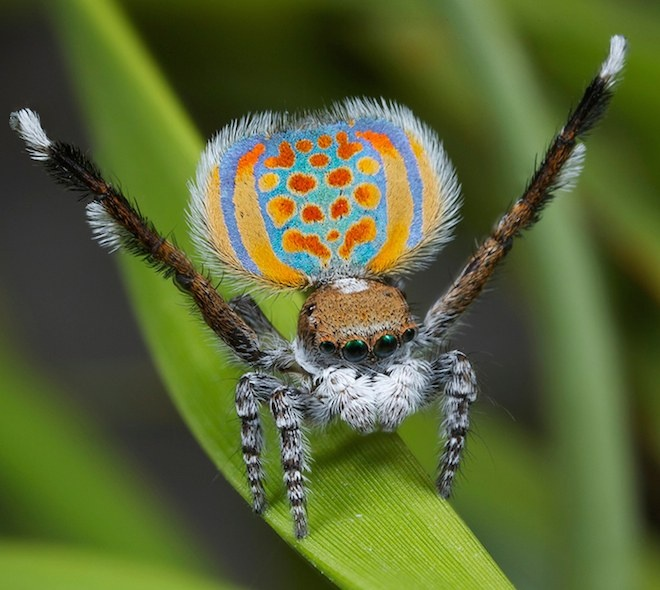
\includegraphics[width=0.49\textwidth]{RGB}
    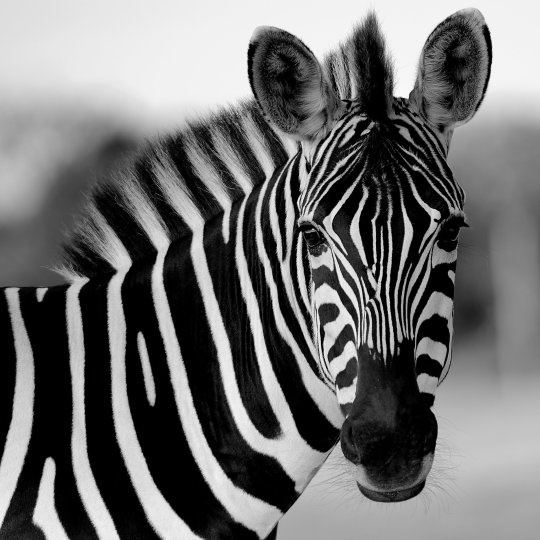
\includegraphics[width=0.49\textwidth]{RGBtoGRAY}
    \caption{A sinistra l'immagine originale. A destra la versione in scala di grigi}
    \label{fig:rgb2gray_example}
  \end{center}
\end{figure}

\subsection {Masking}
La tecnica del \textit{masking} permette di nascondere parti di immagine a cui non siamo interessati.
Abbiamo bisogno di una maschera binaria e dell'immagine che si vuole mascherare.
Per immagine binaria si intende un'immagine in cui ogni \textit{pixel} appartiene all'insieme $\{0,1\}$, cioè è nero oppure bianco.
Solitamente la maschera viene generata a mano con semplici editor.
Si fa notare che quest'ultima deve avere le stesse dimensioni dell'immagine di partenza.
L'operazione consiste nell'effettuare un AND logico, \textit{pixel} per \textit{pixel},  tra l'immagine e la maschera.
Così facendo tutti i \textit{pixel} dell'immagine di partenza corrispondenti a zone di valore $0$ della maschera verranno impostati a $0$, diventando quindi neri.
Il resto dell'immagine non viene alterato.

Nell'esempio in figura~\ref{fig:mask_example} si è deciso di rimuove l'informazione relativa allo sfondo.

\begin{figure}[ht] % TODO
  \begin{center}
  \begin{subfigure}{.49\linewidth}
    \centering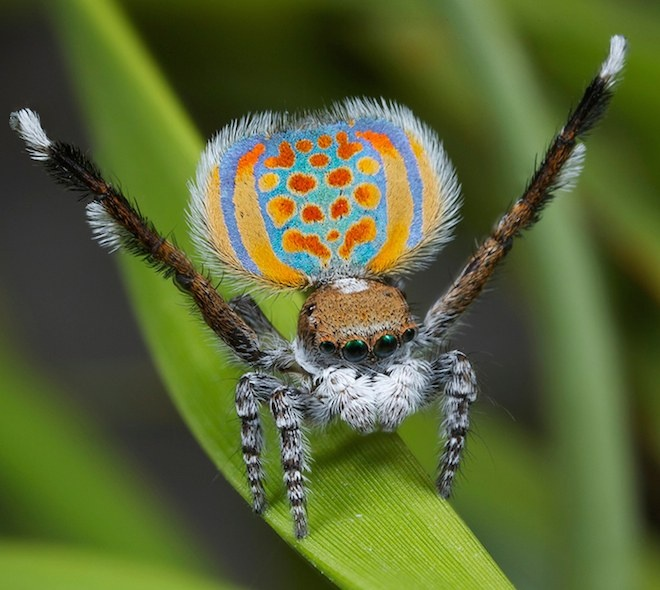
\includegraphics[width=\textwidth]{RGB}
    \caption{Immagine originale}
  \end{subfigure}
  \begin{subfigure}{.49\linewidth}
    \centering
\includegraphics[width=\textwidth]{mask}
    \caption{Maschera binaria}
  \end{subfigure}
  \begin{subfigure}{.49\linewidth}
    \centering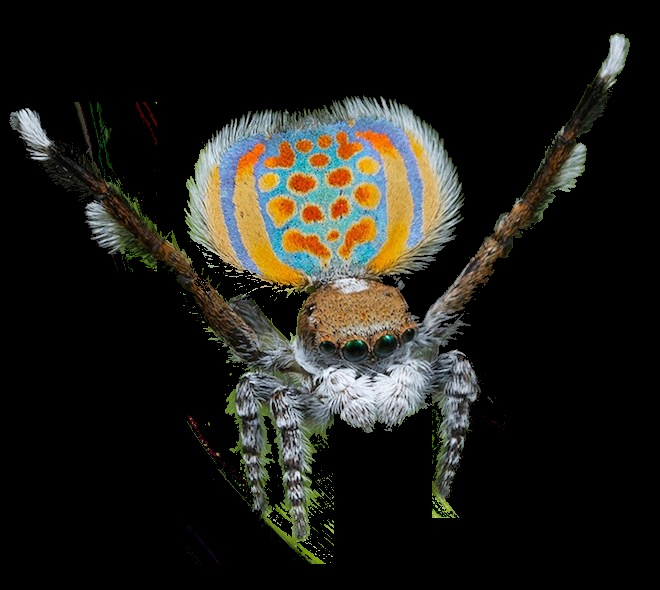
\includegraphics[width=\textwidth]{masked}
    \caption{Risultato del mascheramento}
  \end{subfigure}
  \end{center}
    \caption{Esempio di mascheramento di un'immagine a colori}
    \label{fig:mask_example}
\end{figure}

% TODO dire che ci sono vari tipi di masking?

% \clearpage
% \subsection {Traslazioni e Rotazioni}
% 
% Trasformazioni Affini
% % https://en.wikipedia.org/wiki/Digital_image_processing
% % https://en.wikipedia.org/wiki/Affine_transformation
% % https://en.wikipedia.org/wiki/Rotation
% 
% Come abbiamo accennato prima, le trasformazioni affini ci permettono di effettuare traslazioni e rotazioni alle immagini.
% 
% TODO
% 
% Con la matrice per il cambio di base
% % wrap affine e matrici di traslazione / rotazione
% % cfr cambio di base?
% \begin{figure}[ht] % TODO immagini
%   \begin{center}
%     \includegraphics[width=0.3\textwidth]{example-image}
%     \includegraphics[width=0.2\textwidth]{example-image}
%     \includegraphics[width=0.3\textwidth]{example-image}
%     \caption{TODO cambiare immagini}
%     \label{fig:traslation_example}
%   \end{center}
% \end{figure}

\clearpage
\subsection {Image Cropping and Resizing}
Quando si effettua un \textit{image cropping} si ritaglia una porzione dell'immagine, che viene chiamata ROI (\textit{Region Of Interest}), sulla quale si vuole concentrare l'attenzione.
Dato che ogni immagine è rappresentata con una matrice, una ROI non sarà nient'altro che una matrice di dimensioni minori in cui sono stati copiati i valori dell'area interessata.
Una matrice di questo tipo viene anche chiamata vista o \textit{view}.
% https://en.wikipedia.org/wiki/Cropping_(image)

Con l'\textit{image resizing} si aumentano (o diminuiscono) le dimensioni di un'immagine.
Nel primo caso, poiché si vuole aumentare il numero di \textit{pixel} dell'immagine finale,bisognerà utilizzare tecniche di \textit{upsampling} ed interpolare i dati a disposizione per generarne di nuovi che siano verosimili.

Uno fra gli algoritmi più semplici è \textit{Nearest-Neighbor Interpolation}:
il \textit{pixel} che deve essere aggiunto ottiene il valore del \textit{pixel} a lui più vicino.
Un criterio di scelta dovrà essere definito nel caso in cui ci siano più \textit{pixel} alla stessa distanza ma con valori differenti.
Un criterio possibile è quello di assegnare al nuovo \textit{pixel} il valore del \textit{pixel} alla sua sinistra ed in alto.
% https://en.wikipedia.org/wiki/Nearest-neighbor_interpolation
% https://docs.opencv.org/2.4/modules/imgproc/doc/geometric_transformations.html
% https://en.wikipedia.org/wiki/Image_scaling
% https://en.wikipedia.org/wiki/Scale_(ratio)

Una tecnica leggermente più complessa, ma che fornisce risultati soddisfacenti nella maggior parte delle occasioni, è l'interpolazione bilineare.
Con questa tecnica si effettuano, in cascata, due interpolazioni lineari, una orizzontale ed una verticale.
Con l'interpolazione bilineare i nuovi \textit{pixel} si ottengono come media dei valori noti, pesata rispetto allo loro distanza dal \textit{pixel} che si vuole colorare.
In questo modo si ottengono immagini con transazioni di colore più dolci.
Maggiori informazioni ed immagini esemplificative possono essere trovate, per quanto riguarda l'interpolazione lineare, in \cite{linear-interpolation} e, per l'interpolazione bilineare, in \cite{bilinear-interpolation}.

Nel caso in cui si voglia ridurre le dimensioni dell'immagine si dovranno usare tecniche di \textit{downsampling} ed \textit{anti-aliasing}.
% https://en.wikipedia.org/wiki/Anti-aliasing_filter
Il \textit{downsampling} permette di selezionare un numero limitato di \textit{pixel} che poi verranno usati per colorare la matrice di dimensione ridotta.
Applicare soltanto questa tecnica può portare alla creazione di artefatti sintetici nell'immagine risultato.
Significa che l'immagine ridotta potrebbe contenere gruppi di \textit{pixel} di colori sbagliati.
Sfruttando tecniche come l'\textit{anti-aliasing} si può evitare, o quantomeno limitare, la creazione di tali artefatti.
Un \textit{low-pass filter} è un tipo di filtro che smorza tutti i valori al di sopra di una certa soglia, mentre lascia passare tutti i valori al di sotto.
Nel campo dell'elaborazione digitale delle immagini vengono utilizzati filtri di \textit{blur} applicati tramite convoluzione.
Il termine \textit{blur} o \textit{smooth} indica applicare un effetto sfocato, che tende a rendere più dolci le transizioni da un colore all'altro.
Andando quindi anche a ridurre valori troppo alti (o troppo bassi) avvicinandoli a valori più probabili.


\clearpage
\subsection {Histogram Equalization}
Citando Wikipedia~\cite{wikipedia-hist-eq}:
\begin{quote}
  \textit{Histogram equalization is a method in image processing of contrast adjustment using the image's histogram.}
\end{quote}
Si ricorda che il contrasto è definito come la differenza in intensità luminosa e colore che permette di distinguere gli oggetti in un'immagine.
In figura~\ref{fig:hist_eq_example} sono stati riporta un'immagine a basso contrasto e l'immagine risultato dopo l'applicazione della \textit{histogram equalization}.
Nella figura si possono osservare anche gli istogrammi relativi alle immagini: sull'asse delle $x$ abbiamo ogni possibile valore di un \textit{pixel}, quindi nell'intervallo da 0 a 255; sull'asse delle $y$ è riportato il numero di occorrenze di quel colore nell'immagine.
Notare che l'immagine in ingresso deve essere in scala di grigi.

Vediamo ora come la costruzione dell'istogramma e la sua manipolazione possono essere formulate matematicamente.
Siano $X$ l'immagine di partenza ed $Y$ l'immagine risultato.
Facendo riferimento a quanto scritto nel documento~\cite{hist-eq} l'istogramma può essere definito come:
\begin{equation*}
p_n = \frac{\text{numero di pixel di colore $n$}}{\text{numero totale di pixel}} \quad \text{con $n$} \in [0,255]
\end{equation*}
Poiché $p_n$ descrive la probabilità che un \textit{pixel}, scelto a caso dall'immagine, abbia valore $n$, possiamo considerare $X$ una variabile casuale discreta in $[0,255]$.
Quindi $X$ avrà funzione di ripartizione, tracciata in blu nel grafico in figura~\ref{fig:hist_pre_eq_example}, pari ad:
\begin{equation*}
  F_X(x) = \sum_{n=0}^{x} p_n
\end{equation*}
Vorremmo che la differenza di colore tra i pixel fosse più netta, così da aumentare il contrasto dell'immagine.
Per raggiungere i nostri scopi possiamo ridistribuire equamente i valori di $X$ nell'intervallo dei valori possibili:
\begin{equation*}
  T(x) = \text{floor}(255 * F_X(x))
\end{equation*}
dove floor() arrotonda verso il basso all'intero più vicino.
In questo modo possiamo ottenere la variabile casuale trasformata $Y=T(X)$, ossia l'immagine equalizzata.
Sostanzialmente abbiamo ricolorato ogni pixel dell'immagine di partenza con colori più distanti tra loro, come si può vedere nell'istogramma in figura~\ref{fig:hist_post_eq_example}.

\clearpage
\begin{figure}[ht]
  \begin{center}
  \begin{subfigure}{.49\linewidth}
    \centering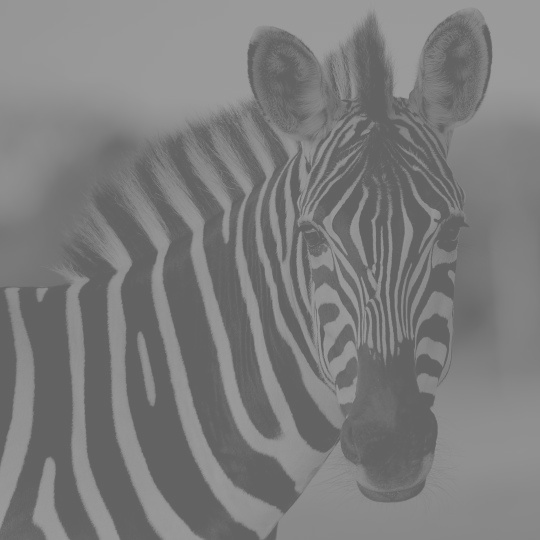
\includegraphics[width=\textwidth]{GRAY_low_contrast}
    \caption{Immagine originale}
  \end{subfigure}
  \begin{subfigure}{.49\linewidth}
    \centering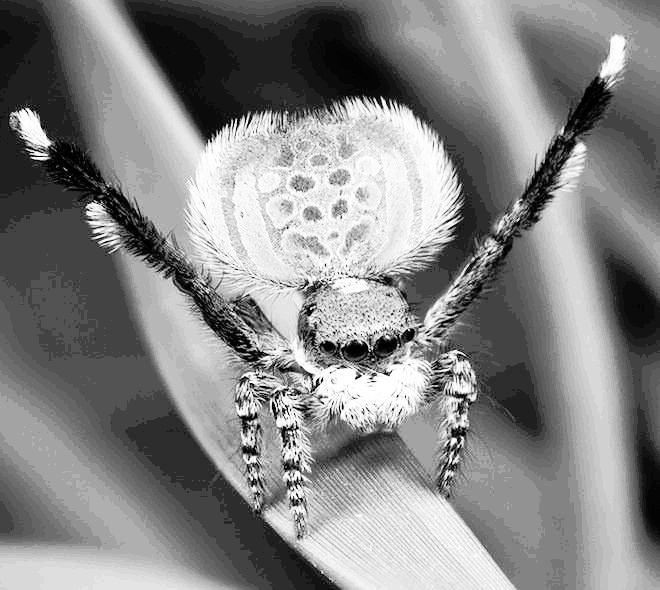
\includegraphics[width=\textwidth]{eqHist_example}
    \caption{Immagine equalizzata}
  \end{subfigure}
  \begin{subfigure}{.73\linewidth}
    \centering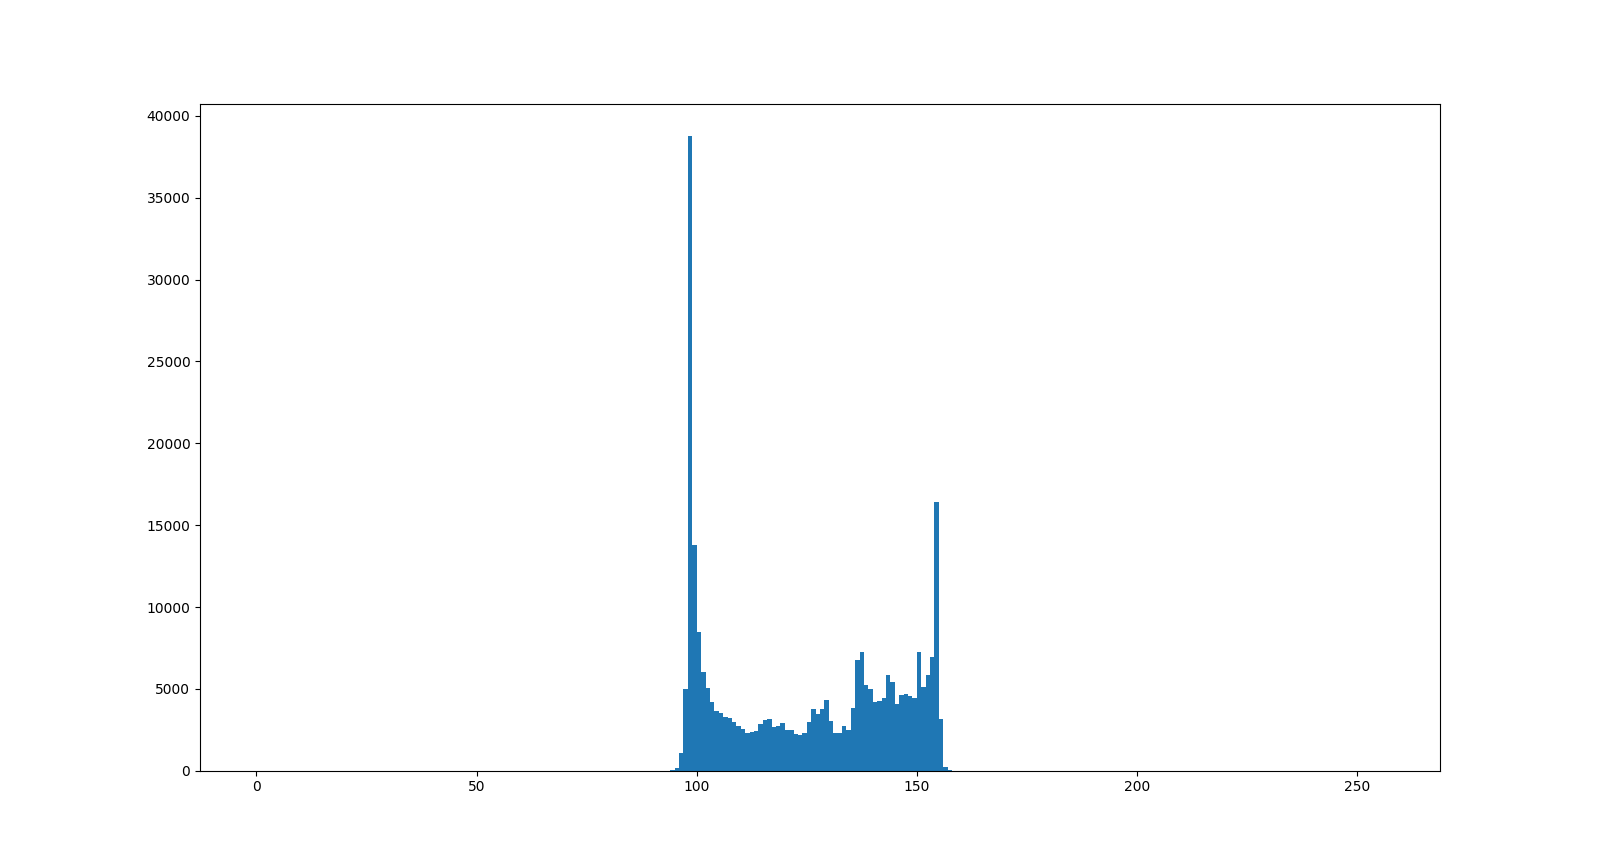
\includegraphics[width=\textwidth]{pre_eq_hist}
    \caption{Istogramma dell'immagine originale}
    \label{fig:hist_pre_eq_example}
  \end{subfigure}
  \begin{subfigure}{.73\linewidth}
    \centering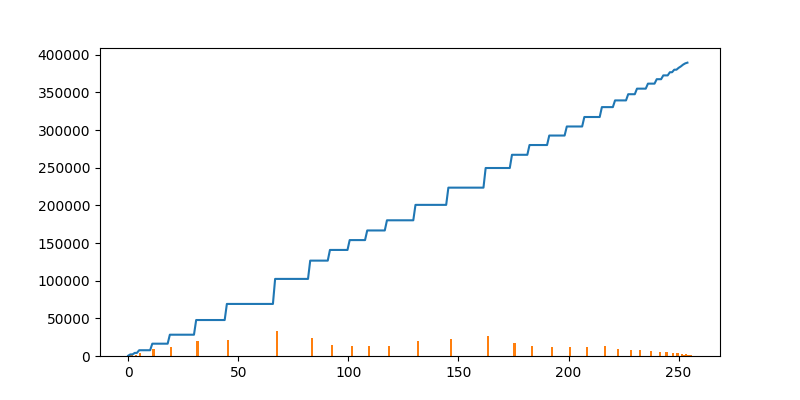
\includegraphics[width=\textwidth]{post_eq_hist}
    \caption{Istogramma dell'immagine equalizzata}
    \label{fig:hist_post_eq_example}
  \end{subfigure}
  \end{center}
    %\caption{TODO rifare grafici}
  \caption{Esempio di applicazione di \textit{histogram equalization}}
    \label{fig:hist_eq_example}
\end{figure}

\clearpage
\subsection {Gaussian Blur}
Conosciuto anche come \textit{Gaussian smoothing}, il \textit{Gaussian blur} permette di sfocare un immagine sfruttando una convoluzione con \textit{kernel} gaussiano.
L'immagine così ottenuta risulta meno nitida, con meno dettagli e, quindi, con meno rumore.
L'obbiettivo principale di questa tecnica è mantenere soltanto l'informazione caratterizzante, rimuovendo quella non necessaria od anomala.
%Si può dimostrare che il \textit{Gaussian blur} è un \textit{low-pass filter}.
Si ricorda che la funzione di Gauss ad un parametro è
\begin{equation*}
  G(x) = \frac{1}{\sqrt{2\pi\sigma^2}}
         \exp{\Bigl(- \frac{ x^2 }{ 2 \sigma^2 } \Bigr)} 
\end{equation*}
Si dimostra che la funzione di Gauss a due parametri equivale al prodotto di due funzioni come quella appena definita, in formule
\begin{equation*}
  \begin{split}
    G(x,y) & = G(x)G(y) \\
           & = \frac{1}{2\pi\sigma^2}
               \exp{\Bigl(- \frac{ x^2 + y^2 }{ 2 \sigma^2 } \Bigr)} 
  \end{split}
\end{equation*}
in cui $x$ ed $y$ sono le distanze dagli assi di riferimento, mentre $\sigma$ è la deviazione standard.
% In termini di calcolo computazionale ciò può essere sfruttato eseguendo due computazioni lineari,
% rispetto alle dimensioni dell'immagine e del kernel, %non corretto
% \todo{TODO correggere e dire meglio}
% anziché una quadratica.
% 
% $
% {\displaystyle O\left(w_{\text{kernel}}w_{\text{image}}h_{\text{image}}\right)+O\left(h_{\text{kernel}}w_{\text{image}}h_{\text{image}}\right)}
% $
% 
% $
% {\displaystyle O\left(w_{\text{kernel}}h_{\text{kernel}}w_{\text{image}}h_{\text{image}}\right)}
% $

La matrice sottostante rappresenta un'approssimazione di un filtro gaussiano quadrato di lato $7$ con $\sigma = 2$.

\begin{equation*} % TODO 
  \frac{1}{100}*
  \begin{bmatrix}

    0.5 & 0.9 & 1.3 & 1.5 & 1.3 & 0.9 & 0.5\\
    0.9 & 1.7 & 2.4 & 2.8 & 2.4 & 1.7 & 0.9\\
    1.3 & 2.4 & 3.6 & 4.0 & 3.6 & 2.4 & 1.3\\
    1.5 & 2.8 & 4.0 & 4.6 & 4.0 & 2.8 & 1.5\\
    1.3 & 2.4 & 3.6 & 4.0 & 3.6 & 2.4 & 1.3\\
    0.9 & 1.7 & 2.4 & 2.8 & 2.4 & 1.7 & 0.9\\
    0.5 & 0.9 & 1.3 & 1.5 & 1.3 & 0.9 & 0.5

  \end{bmatrix}
\end{equation*}
\label{eq:gauss_kernel}
% http://dev.theomader.com/gaussian-kernel-calculator/

Ricordiamo che durante una convoluzione si effettua la somma dei prodotti elemento per elemento, ossia una media pesata in cui i pesi sono definiti nel kernel.
Dato che i valori al centro del filtro sono più grandi di quelli ai bordi, daremo maggior peso ai pixel nell'intorno dell'elemento su cui il kernel viene centrato.
All'aumentare di $\sigma$ cresce il raggio alla base della campana di Gauss, questo significa che, con $\sigma$ grandi, verrà data importanza anche ai pixel distanti.
Ciò farà risultare l'immagine in uscita molto più sfocata.

In figura~\ref{fig:gaussian_blur_example} è riportata un'immagine prima e dopo l'applicazione del filtro riportato in \ref{eq:gauss_kernel}, si fa notare come i dettagli più piccoli sono stati rimossi, mentre l'oggetto dell'immagine rimane distinguibile.

\begin{figure}[ht] % TODO
  \begin{center}
    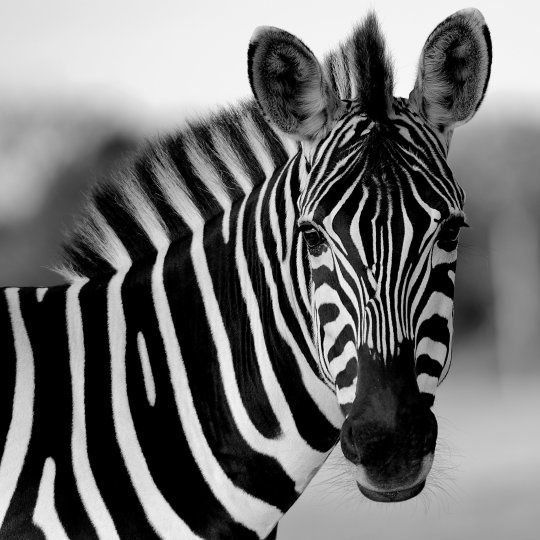
\includegraphics[width=0.49\textwidth]{GRAY}
    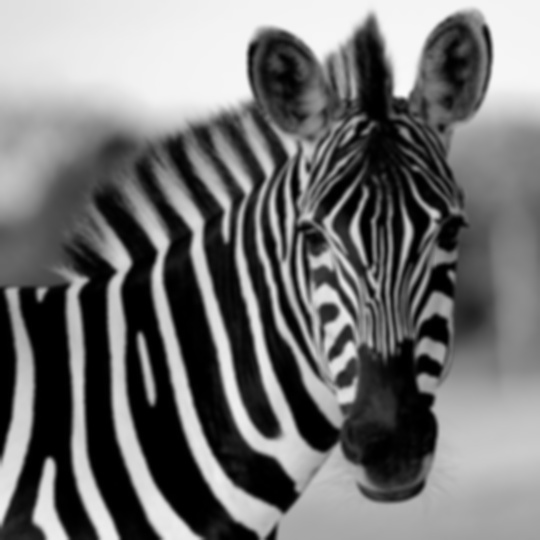
\includegraphics[width=0.49\textwidth]{gaussian_blur_example}
    \caption{A sinistra l'immagine originale. A destra il risultato del \textit{blur}}
    \label{fig:gaussian_blur_example}
  \end{center}
\end{figure}

%Va fatta un'ultima considerazione: cosa succede se applico due volte lo stesso filtro?
%Se si applica più volte uno stesso filtro gaussiano si ottiene lo stesso risultato che si otterrebbe dopo un'unica applicazione di un filtro 
%\todo{TODO completare}

%\clearpage
%\subsection {Bilateral Filter}
%TODO
% https://en.wikipedia.org/wiki/Bilateral_filter
% https://docs.opencv.org/2.4/modules/imgproc/doc/filtering.html?highlight=bilateralfilter#bilateralfilter

% Capire formule in 
% http://homepages.inf.ed.ac.uk/rbf/CVonline/LOCAL_COPIES/MANDUCHI1/Bilateral_Filtering.htmlhttp://homepages.inf.ed.ac.uk/rbf/CVonline/LOCAL_COPIES/MANDUCHI1/Bilateral_Filtering.html


%\clearpage
\subsection {Sobel Operator}
Prima di descrivere cosa sia il \textit{Sobel operator}, detto anche filtro Sobel, bisogna dare una definizione di gradiente.
% TODO formattare correttamente la citazione
Nel calcolo vettoriale, il gradiente è la generalizzazione della derivata.
La derivata di una funzione ad una variabile associa ad ogni punto uno scalare, mentre il gradiente di una funzione a più variabili $f$ associa ad ogni punto un vettore multidimensionale.
Quest'ultimo è composto dall'insieme delle derivate parziali di $f$ nel punto considerato.
Il gradiente rappresenta la pendenza della tangente al grafico della funzione in un punto.
La sua direzione indica il più grande incremento della funzione mentre il modulo\footnote{Detto \textit{magnitude} in inglese.} è il tasso d'incremento.

Possiamo pensare un'immagine (in scala di grigi) come una funzione a due variabili che associa ad ogni punto $(x,y)$ un valore in $[0,255]$.
Il gradiente dell'immagine sarà composto da vettori direzionati in modo da uscire dalle zone scure ed entrare nelle zone più chiare (mantenendo la convenzione per cui a zero è associato il colore nero).
La magnitudine sarà tanto più grande quanto più grande il contrasto, quindi la differenza di colore e luminosità.
%In figura~\ref{fig:gradient} è presentato un esempio di gradiente di un'immagine.
%\begin{figure}[ht] % TODO
%  \begin{center}
%    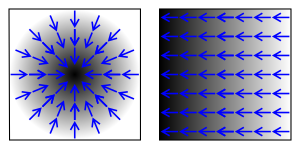
\includegraphics[width=0.2\textwidth]{gradient}
%    \caption{TODO occhio che qui black=high e white=low}
%    \label{fig:gradient}
%  \end{center}
%\end{figure}

Ora possiamo procedere con la descrizione del filtro di Sobel, facendo riferimento a quanto scritto in \cite{wikipedia-sobel}.
Il \textit{Sobel filter} viene utilizzato per creare immagini in cui si enfatizzano gli \textit{edge}.
Per \textit{edge} si intendono tutte quelle zone dell'immagine che corrispondono a bordi, margini o spigoli degli oggetti rappresentati nell'immagine.
Ciascuna di queste zone deve necessariamente essere associata almeno ad un cambio di colore oppure ad un cambio di luminosità, altrimenti l'oggetto in questione non sarebbe distinguibile dallo sfondo.
Quindi, osservando il gradiente dell'immagine, ad ogni \textit{edge} corrisponderà una serie di vettori con modulo più grande rispetto ai moduli dei vettori circostanti.
Lo scopo del filtro Sobel è generare un'approssimazione del gradiente dell'immagine sfruttando due convoluzioni distinte con uno specifico kernel.
Nonostante il risultato sia abbastanza grossolano, la sua efficacia e rapidità lo rendono uno dei principali strumenti per la \textit{edge detection}, tecnica che esploreremo fra poco.

L'applicazione del filtro Sobel avviene come mostrato nelle equazioni \ref{eq:sobel_gx} e \ref{eq:sobel_gy}, dove $*$ denota una convoluzione ed $I$ è un'immagine in scala di grigi.

\begin{equation} \label{eq:sobel_gx}
  G_x = 
  I
  *
  \begin{bmatrix}
    -1&0&1\\
    -2&0&2\\
    -1&0&1\\
  \end{bmatrix}
\end{equation}
\begin{equation} \label{eq:sobel_gy}
  G_y = 
  I
  *
  \begin{bmatrix}
    -1&-2&-1\\
    0&0&0\\
    1&2&1\\
  \end{bmatrix}
\end{equation}
% TODO allineare le equazioni
L'equazione~\ref{eq:sobel_gx} fornisce un'approssimazione del gradiente rispetto all'asse $x$, mentre l'equazione~\ref{eq:sobel_gy} rispetto ad $y$.
L'equazione~\ref{eq:sobel_g}, invece, combina le precedenti fornendo informazione riguardo al modulo del gradiente dell'immagine.
Con l'equazione~\ref{eq:sobel_angle} si ottiene la direzione del gradiente.
% TODO c'è un modo per non ripetere "equazione" tante volte?
\begin{equation} \label{eq:sobel_g}
  G = \sqrt{G_x^2 + G_y^2}
\end{equation}
\begin{equation} \label{eq:sobel_angle}
  \Theta = atan{\Bigl( \frac{G_y}{G_x} \Bigr)}
\end{equation}

Ora verranno fatte delle considerazioni sul kernel mostrato nella formula~\ref{eq:sobel_gx}.
Poiché il filtro nell'equazione~\ref{eq:sobel_gy} è una semplice trasposta del precedente, tali considerazioni sono, facendo riferimento all'asse delle $y$, valide anche per questo filtro.
Il kernel nell'equazione~\ref{eq:sobel_gx} assegnerà valori in assoluto più grandi a \textit{pixel} in una posizione di transizione di colore, rispetto a \textit{pixel} posizionati in una zona con colorazione uniforme.
%TODO forse si può dire meglio
Prendiamo un \textit{pixel} $p$ di colore bianco posizionato in una zona in cui tutti i \textit{pixel} sono di colore bianco, si avrà che il \textit{kernel}, pesando i \textit{pixel} a destra allo stesso modo di quelli a sinistra ma con segno opposto, attribuisce un valore pari a $0$ a $p$.
Se $p$ fosse stato in una zona si transizione dal bianco al nero, avrebbe ottenuto un valore negativo molto grande:
tutti i valori nella prima colonna del filtro sarebbero stati moltiplicati per $255$ mentre tutti quelli dell'ultima colonna sarebbero stati annullati, essendo moltiplicati per $0$.
Uno stesso ragionamento può essere effettuato considerando zone completamente nere oppure di transizione dal nero al bianco.

Nell'immagine sottostante viene mostrata l'applicazione dell'operatore Sobel prima rispetto ad $x$, poi rispetto ad $y$ ed infine il risultato della combinazione delle precedenti.

%\begin{figure}[ht] % TODO
%  \begin{center}
%    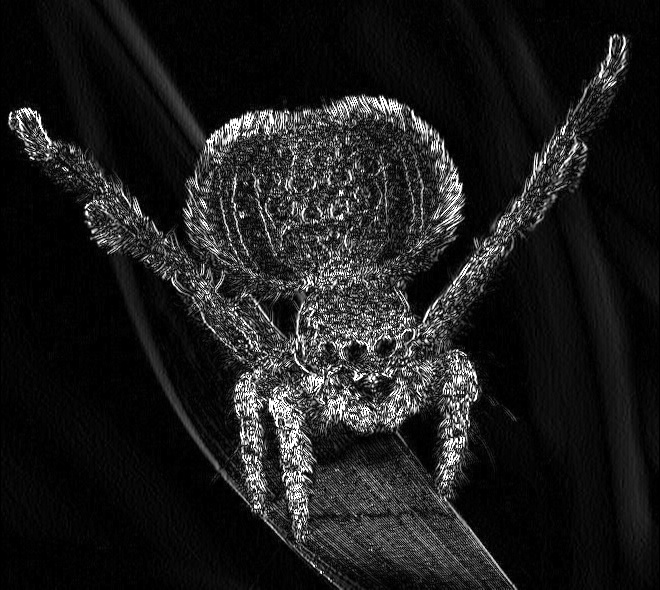
\includegraphics[width=0.3\textwidth]{gx}
%    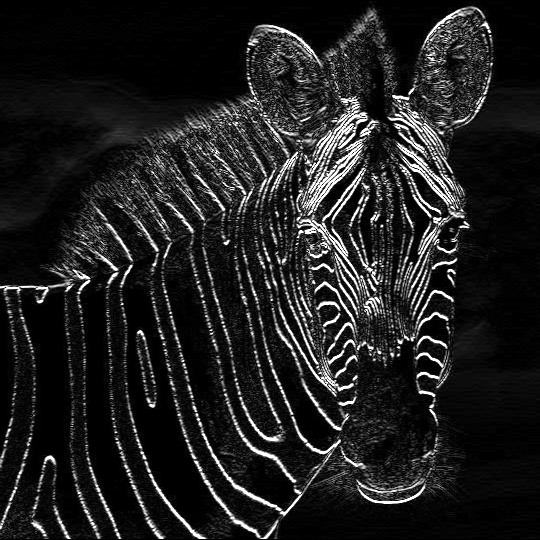
\includegraphics[width=0.3\textwidth]{gy}
%    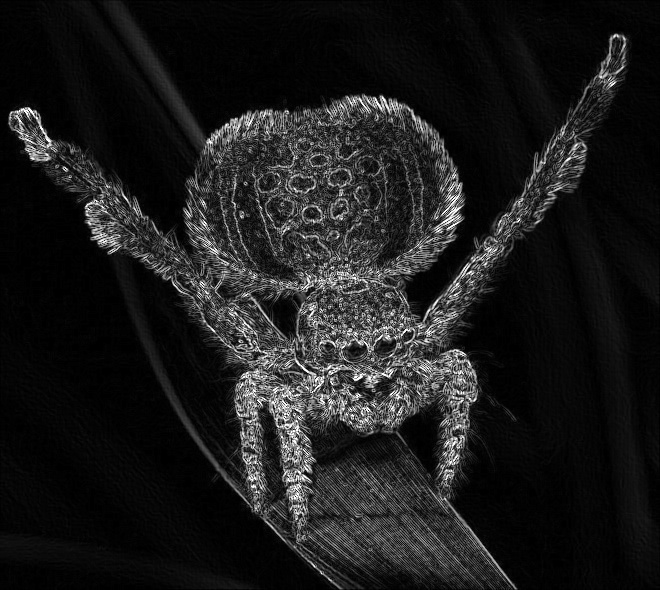
\includegraphics[width=0.3\textwidth]{g}
%    \caption{TODO caption}
%    \label{fig:sobel_example}
%  \end{center}
%\end{figure}

\begin{figure}[ht]
  \begin{center}
  \begin{subfigure}{.49\linewidth}
    \centering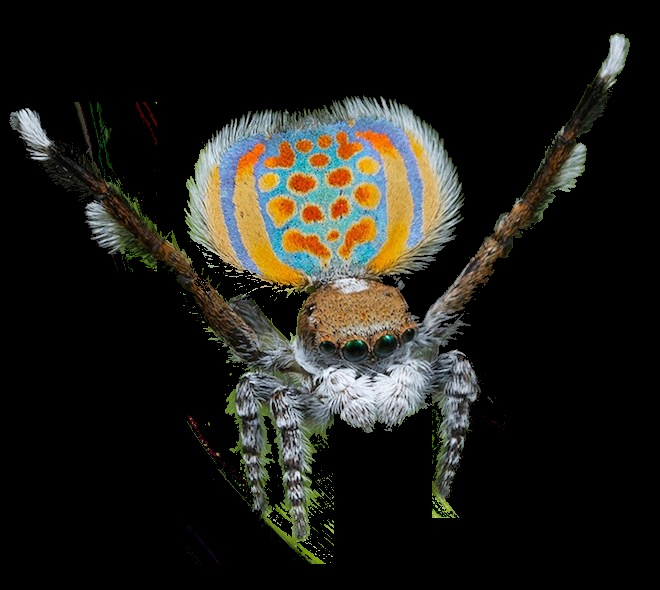
\includegraphics[width=\textwidth]{masked}
    \caption{Immagine originale}
  \end{subfigure}
  \begin{subfigure}{.49\linewidth}
    \centering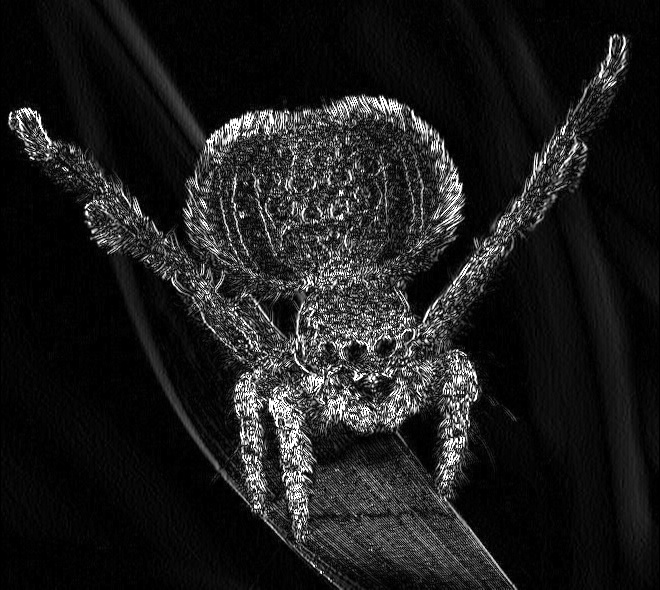
\includegraphics[width=\textwidth]{gx}
    \caption{Risultato rispetto ad $x$}
  \end{subfigure}
  \begin{subfigure}{.49\linewidth}
    \centering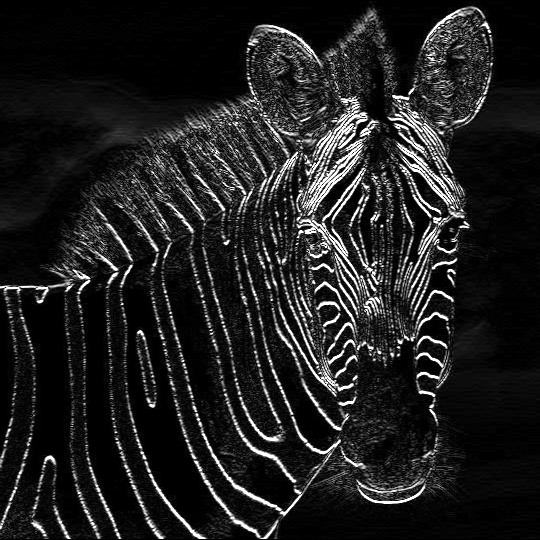
\includegraphics[width=\textwidth]{gy}
    \caption{Risultato rispetto ad $y$}
  \end{subfigure}
  \begin{subfigure}{.49\linewidth}
    \centering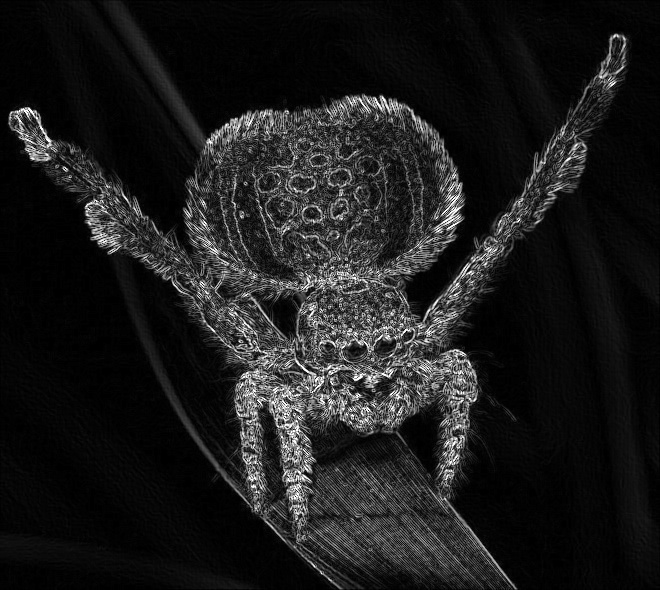
\includegraphics[width=\textwidth]{g}
    \caption{Risultato combinato}
  \end{subfigure}
  \end{center}
  \caption{Esempio di applicazione del filtro Sobel}
    \label{fig:sobel_example}
\end{figure}


\clearpage
\subsection {Canny Edge Detector}
Composto da vari passaggi ed algoritmi, il \textit{Canny Edge Detector} permette di estrarre i principali \textit{edge} di un'immagine ottenendo risultati soddisfacenti ed adattabili alle necessità dell'utilizzatore.
Questo rilevatore viene sfruttato largamente come tecnica di estrazione delle caratteristiche perché permette di rimuovere molta informazione dall'immagine, mantenendo solo quella strettamente necessaria.
Nell'ambito del \textit{edge detection} è bene che tutti gli \textit{edge} presenti nell'immagine vengano identificati correttamente, ma è altrettanto importante che non vengano generati falsi positivi, cioè che delle aree nel risultato presentino contorni che nell'immagine di partenza non esistevano.
Per questo motivo \textit{Canny edge detector} effettua molte operazioni di rimozione di falsi positivi ed allo stesso tempo tende ad evidenziare molto bene quelli che sembrano essere \textit{edge} autentici.
Ora verranno elencati in ordine i vari passaggi del rilevatore:
\begin{enumerate}
  \item Viene applicato un filtro gaussiano per effettuare uno \textit{smooth} all'immagine.
    Questo passaggio è fondamentale perché vengono rimossi valori anomali che, risultando come picchi positivi o negativi, potrebbero contribuire a generare falsi positivi.
    Inoltre può essere usato per rimuovere dettagli superflui.

  \item Utilizzando il filtro Sobel si ottiene il modulo dei gradienti dell'immagine, ossia tutti gli \textit{edge} candidati, che dovranno poi essere manipolati e selezionati.

  %\item Con il \textit{non-maximum suppression}  % TODO fare se c'e spazio

  \item Con una doppia sogliatura si ottengono due effetti:
    come prima cosa vengono rimossi tutti quegli edge con magnitudine troppo bassa, perché considerati rumore;
    successivamente gli edge sopravvissuti vengono classificati come forti e deboli, questa informazione verrà sfruttata nel prossimo passaggio.
    Effettuare una sogliatura significa semplicemente osservare ogni valore di un'immagine (nel nostro caso ogni \textit{pixel} indica il modulo del gradiente) e mapparlo ad un valore dato se soddisfa determinate condizioni.
    In questo passaggio sono presenti due soglie.
    La prima ci permette di annullare tutti gli edge con valori troppo piccoli.
    La seconda viene usata per etichettare i \textit{pixel} superiori alla soglia come \textit{edge} forti.
    Tutti i \textit{pixel} intermedi vengono considerati \textit{edge} deboli.

  \item A questo punto si procede con il rimuovere tutti gli \textit{edge} deboli che non facciamo parte di nessun \textit{edge} forte.
    Significa che, per ogni \textit{pixel} etichettato come \textit{edge} debole, vengono osservati gli otto \textit{pixel} circostanti.
    Se nessuno di questi è un \textit{edge} forte allora il \textit{pixel} centrale viene annullato.
    % TODO cfr Connected Componets

\end{enumerate}
Va fatto notare che i valori delle due soglie devono essere trovati in modo empirico, a seconda del tipo d'immagine bisognerà impostare soglie più o meno grandi, ma anche più o meno distanti fra loro.

In figura~\ref{fig:canny_example} è illustrata l'applicazione del \textit{Sobel operator}, notare come il risultato sia molto più pulito di quello illustrato in figura~\ref{fig:sobel_example}.
\begin{figure}[ht]
  \begin{center}
    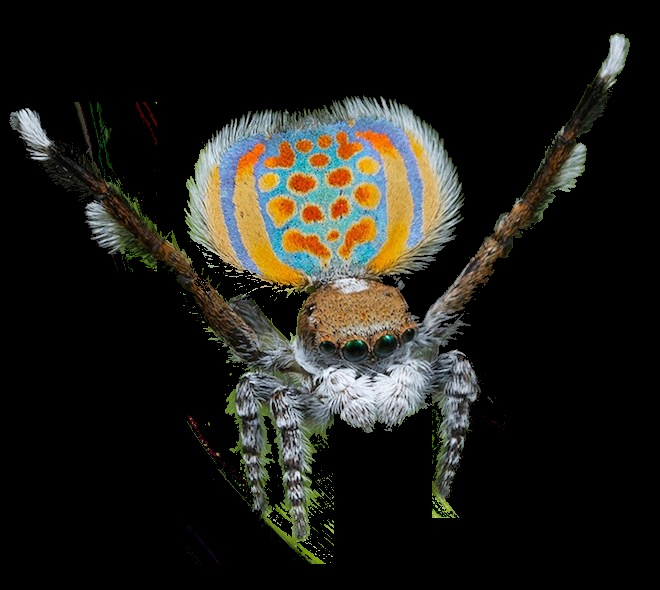
\includegraphics[width=0.49\textwidth]{masked}
    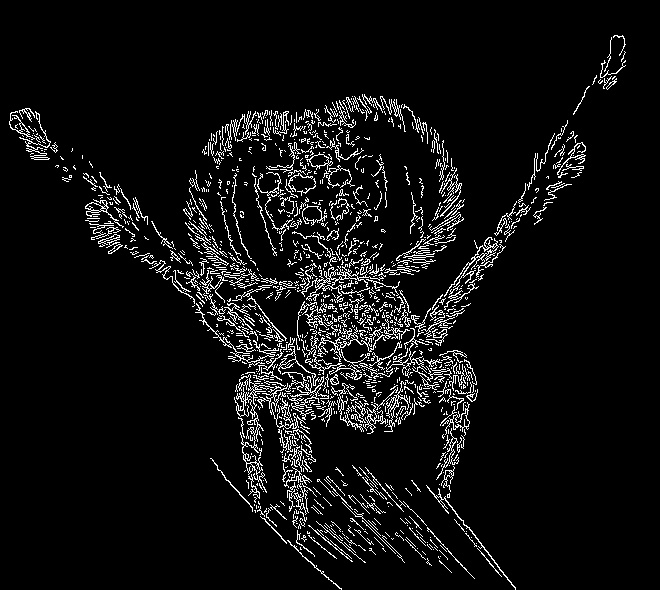
\includegraphics[width=0.49\textwidth]{canny_example}
    \caption{Esempio di applicazione del \textit{Canny Edge Detector}}
    \label{fig:canny_example}
  \end{center}
\end{figure}

\subsection {Hough Circle Transform}
Prima di poter spiegare questa tecnica si devono introdurre alcuni concetti come la \textit{Hough Line Transform}, lo \textit{Hough Parameter Space} e la parametrizzazione raggio-angolo di una retta.
Le trasformate di Hough sono largamente usate come metodi di estrazione delle caratteristiche, permettono di rilevare semplici figure come linee e cerchi.
Il loro obbiettivo è raggruppare correttamente un'insieme di pixel in modo che l'insieme raffiguri la forma che si vuole trovare.
Una delle problematiche principali è la possibilità che nell'immagine la forma da rilevare sia discontinua o deformata.

Esploriamo, facendo riferimento a quanto illustrato in \cite{hough-line}, come il metodo di \textit{Hough Line Transform} permette di trovare una linea retta in un'immagine.
Definiamo tre punti $P_i=(x_i, x_i)$ con $i=1,2,3$ in modo che siano allineati, cioè che esista una retta alla quale appartengano tutti.
Sappiamo che per ciascun punto ci sono infinite rette che soddisfano $y_i = m x_i + c$, ma che soltanto una di queste rette passa anche per gli altri due punti.
L'equazione appena descritta è in funzione di $m$ e $c$, riscrivendola come
\begin{equation} \label{eq:cm_lines}
  c = y_i - m x_i \quad con \quad i=1,2,3
\end{equation}
risulta più facile immaginarla (fissato un $i$) come una retta in uno spazio in cui $c$ è sull'asse delle ordinate e $m$ su quello delle ascisse.
Lo spazio appena descritto prende il nome di \textit{Hough Parameter Space}, in cui ogni punto $(m,c)$ descrive una retta nello spazio di partenza.
Nello spazio dei parametri di Hough, le tre rette della formula \ref{eq:cm_lines} si devono necessariamente incontrare in esattamente un punto, sia $(m_0,c_0)$.
Questo è dovuto al fatto che sappiamo che deve esistere una coppia di parametri per cui la retta $y = m_0 x + c_0$, nello spazio originale, passa per tutti i $P_i$.
L'idea alla base della \textit{Hough Line Transform} è quella di, definito un range di valori per $m$ e per $c$, trovare quello che soddisfa il maggior numero di equazioni.
In pratica ad ogni cella nello spazio $m$-$c$ viene associato un intero che indica quante delle rette di equazione~\ref{eq:cm_lines} passano per quella cella.

Ci si accorge facilmente che questo metodo non ci permette di rilevare rette parallele all'asse delle $y$, infatti bisognerebbe avere un parametro $m$ con valore che tende all'infinito.
Per risolvere questa problematica viene usata la parametrizzazione raggio-angolo.
Come si vede in figura~\ref{fig:hough_parametr_parametr}, ogni retta viene identificata da una coppia univoca $(r,\theta)$.
Nella coppia $r$ indica la distanza dall'origine al punto più vicino della retta, mentre $\theta$ indica l'angolo tra il segmento appena generato e l'asse delle $x$.
Ogni retta viene identificata dall'equazione:
\begin{equation} \label{eq:raggio_angolo_parametr}
  r = x_i cos \theta + y_i sin \theta \quad con \quad i=1,2,3
\end{equation}
ottenibile con semplici calcoli geometrici.
Questo significa che il fascio di rette nello spazio di partenza verrà descritto da curve nello spazio dei parametri di Hough con assi $\theta$-$r$, come si vede in figura~\ref{fig:hough_parametr_curve}.
Valutando le celle nello stesso modo di prima si ottiene la retta passante per i tre punti ma identificata dalla coppia $(r_0,\theta_0)$.

\begin{figure}[ht]
  \begin{center}
    \begin{subfigure}{.4\linewidth}
      \centering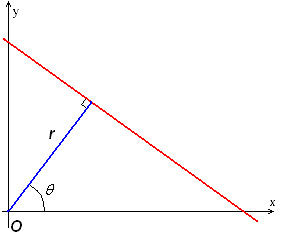
\includegraphics[width=\textwidth]{raggio_angolo}
      \caption{}
      \label{fig:hough_parametr_parametr}
    \end{subfigure}
    \begin{subfigure}{.4\linewidth}
      \centering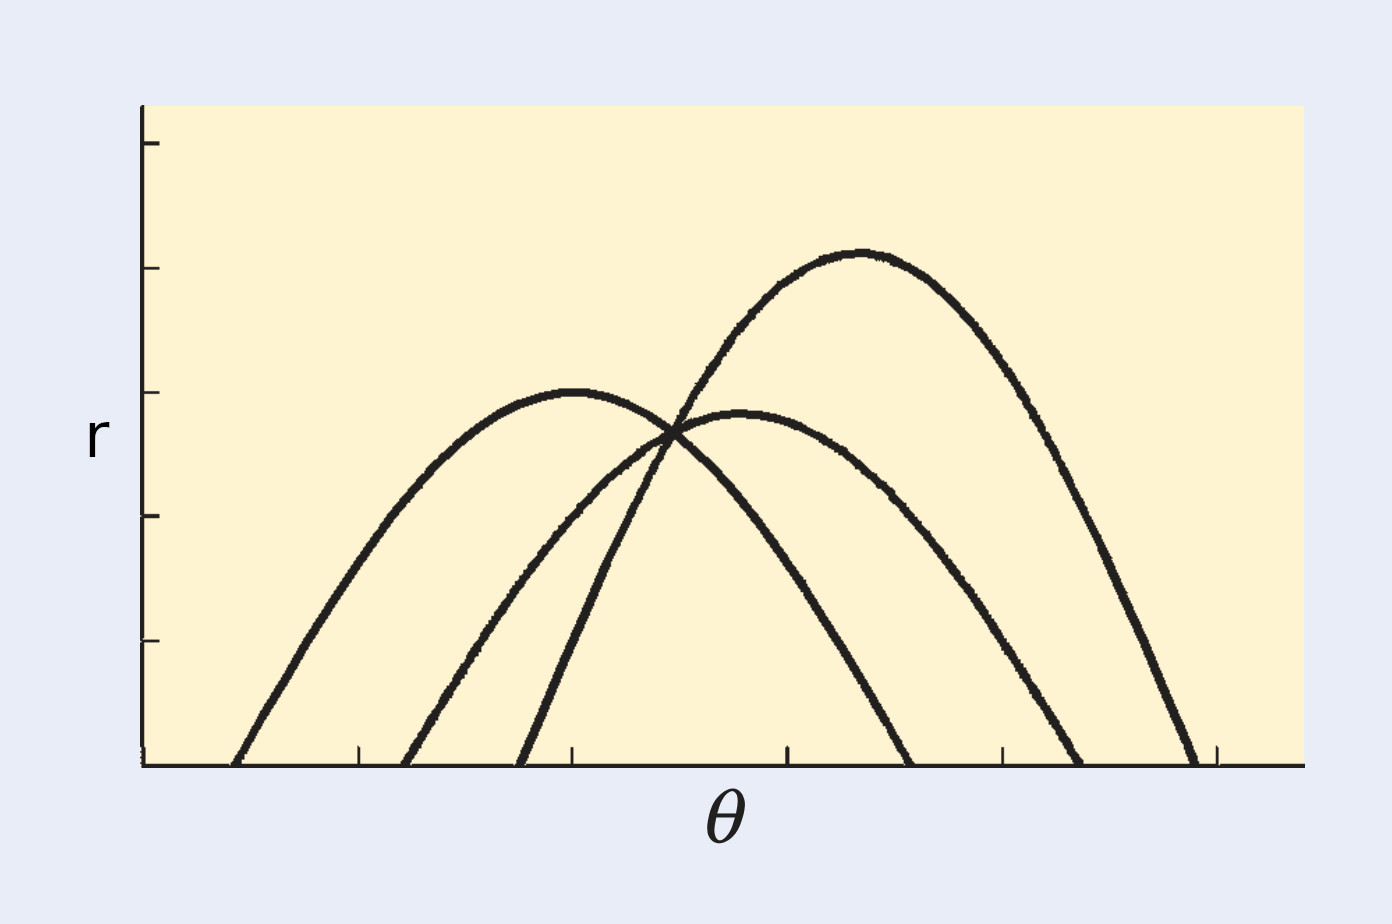
\includegraphics[width=\textwidth]{raggio_angolo_sp}
      \caption{}
      \label{fig:hough_parametr_curve}
    \end{subfigure}
  \end{center}
  \caption{Parametrizzazione raggio-angolo e rappresentazione dello spazio dei parametri di Hough}
  \label{fig:hough_parametr_raggio-angolo}
\end{figure}

Vediamo ora come si può modificare la tecnica appena descritta per rilevare cerchi anziché linee rette.
L'idea principale ruota sempre attorno al concetto di voto di celle nello spazio dei parametri.

In questo caso si sfrutta il fatto che, in una circonferenza $c$ di raggio $r$, ogni punto è equidistante dal centro.
Per ogni punto $P_i$ di $c$ può essere tracciata una circonferenza $c_i$ di centro $P_i$ e raggio $r$.
Sappiamo che tutte le circonferenze $c_i$ si incontrano in un unico punto, il centro di $c$, perché è l'unico equidistante da tutti i centri delle $c_i$.

Si ricorda che l'equazione di una circonferenza di centro $(a,b)$ e raggio $r$ è
\begin{equation} \label{eq:circonferenza}
  (x - a)^2 + (y - b)^2 = r^2
\end{equation}
Supponiamo di conoscere il raggio $r_0$ della circonferenza che vogliamo rilevare e di avere un insieme di punti $P_i$ che sappiamo appartenere alla circonferenza.
Lo spazio dei parametri $a$-$b$ ci permette di creare le circonferenze centrate nei $P_i$ e di assegnare un punteggio alto alla cella in $(a_0,b_0)$ perché votata da molte circonferenze.
In figura~\ref{fig:hough_parametr_circ} si vede la griglia su cui vengono votate le circonferenze.

Se anche il raggio fosse incognito allora lo spazio dei parametri di Hough avrebbe tre dimensioni ed ogni punto sarebbe una tripla $(a,b,r)$ appartenente alla superficie di un cono.

Le implementazioni della \textit{Hough Circle Transform} sfruttano una matrice di supporto, chiamata accumulatore, che corrisponde allo spazio dei parametri di Hough.
Ciascun elemento è un intero con valore iniziale zero, che verrà incrementato di uno per ogni linea passante per quelle coordinate.
\begin{figure}[ht]
  \begin{center}
      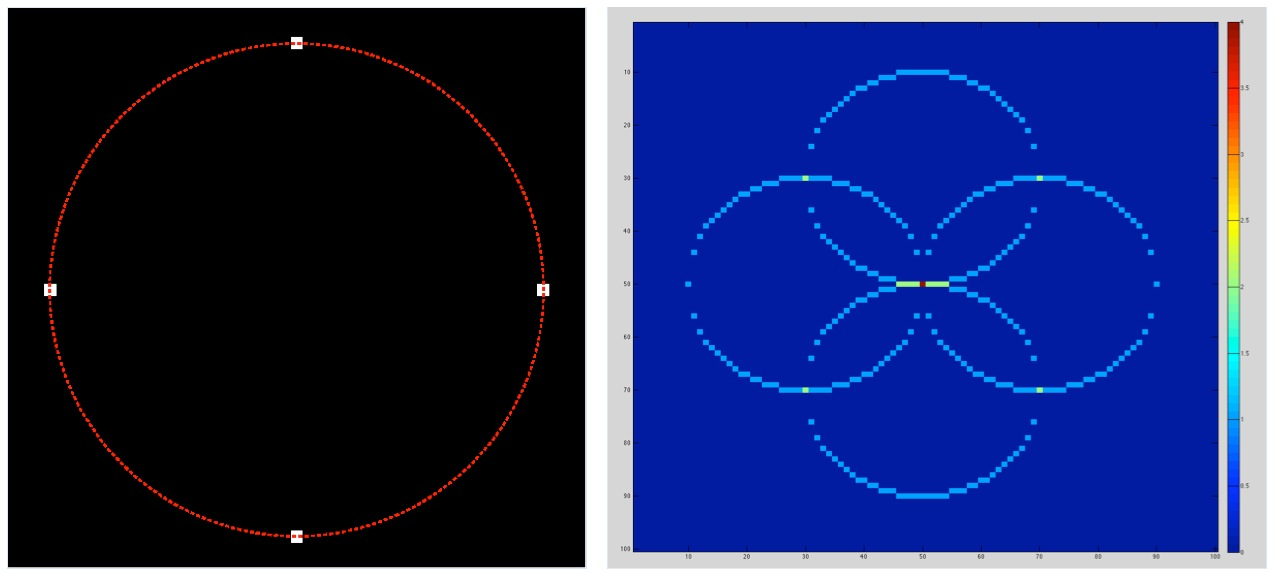
\includegraphics[width=0.75\textwidth]{circle_hough_parameter}
      \caption{Circonferenza e spazio dei parametri di Hough per le circonferenze con raggio dato}
      \label{fig:hough_parametr_circ}
  \end{center}
\end{figure}

% TODO commento sulla implementazione 
% - immagine deve essere canny edge
% - threshold per fare pochi FP
% - min e max radius per restringere la ricerca

% Risorse
% https://docs.opencv.org/2.4/doc/tutorials/imgproc/imgtrans/hough_circle/hough_circle.html
% https://en.wikipedia.org/wiki/Hough_transform
% https://en.wikipedia.org/wiki/Circle_Hough_Transform

\clearpage
\subsection {Applicazione degli algoritmi descritti}
Si fa notare che prima di ottenere immagini come quella illustrata in figura~\ref{fig:prima_dopo_prep} e soprattutto prima di essere sicuri che questo è il tipo di immagine migliore per i nostri scopi, sono stati necessari numerosi esperimenti e tentativi.
In particolar modo è stato importante capire che tipo di informazione potesse essere gestita interamente dalla rete neurale e quale invece dovesse essere rimossa o modificata.
Lo scopo del nostro \textit{pre-processing} è quello di fornire un'immagine contenente solo l'informazione necessaria e sufficiente per poter discriminare un pezzo Conforme da uno Scarto.

Nonostante in questa sezione vengano mostrate solo immagini di carcasse conformi, il processo iterativo appena descritto è stato eseguito confrontando costantemente immagini Conformi e Scarto.
Immagini scarto verranno mostrate nella prossima sezione, interamente dedicata a loro.

% https://tex.stackexchange.com/questions/343605/latex-code-for-subcaption-of-image
\begin{figure}[ht] % TODO
  \begin{center}
    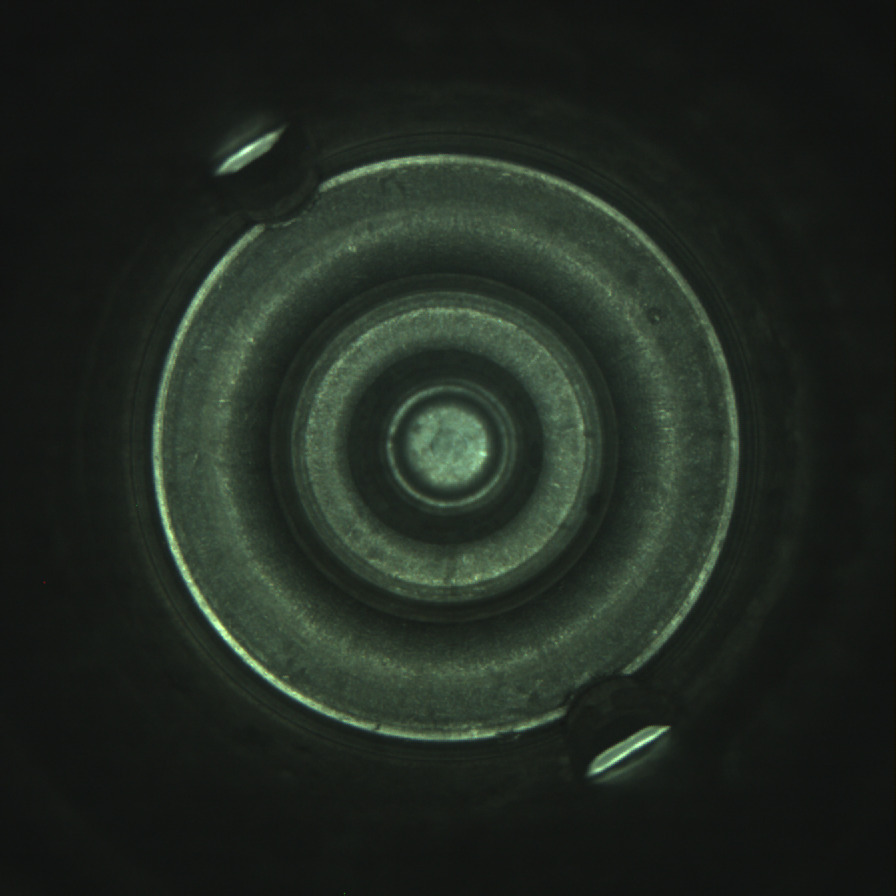
\includegraphics[width=0.5\textwidth]{128___1362_1_1_1_OnLineAnalysis}
    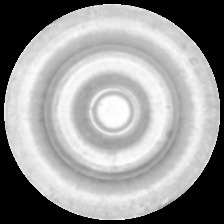
\includegraphics[width=0.35\textwidth]{128___1362_1_1_1_OnLineAnalysis_prep}
    \caption{Un Conforme prima e dopo il \textit{pre-processing}}
    \label{fig:prima_dopo_prep}
  \end{center}
\end{figure}

\subsubsection{1 Centramento con Hough Circle Transform}
Sappiamo che le immagini del \textit{dataset} non sono perfettamente centrate, per questo motivo si è deciso di utilizzare la tecnica della \textit{Hough Circle Transform} per ottenere un'approssimazione del centro della carcassa.
Avendo le coordinate di quest'ultimo si può riallineare il pezzo con il centro dell'immagine.
Ottenere un algoritmo che fosse capace di centrare correttamente tutte le immagini, non è stato facile, ma può essere riassunto nei seguenti passaggi:
\begin{itemize}
  \item creazione di una copia dell'immagine;
  \item conversione della copia in scala di grigi;
  \item equalizzazione dell'istogramma della copia;
  \item ottenimento di alcuni cerchi candidati tramite trasformate di Hough applicate alla copia, qui si sfrutta l'informazione circa le dimensioni tipiche della circonferenza dello scalino più grande;
  \item viene effettuata la media tra i centri dei cerchi ottenuti nel passaggio precedente;
  \item l'immagine originale viene traslata in modo che il centro stimato si trovi in mezzo all'immagine;
\end{itemize}

Nella figura~\ref{fig:centramento} sono illustrati l'immagine prima e dopo il centramento ed il cerchio rilevato.

\begin{figure}[ht] % TODO
  \begin{center}
    \begin{subfigure}{.49\linewidth}
      \centering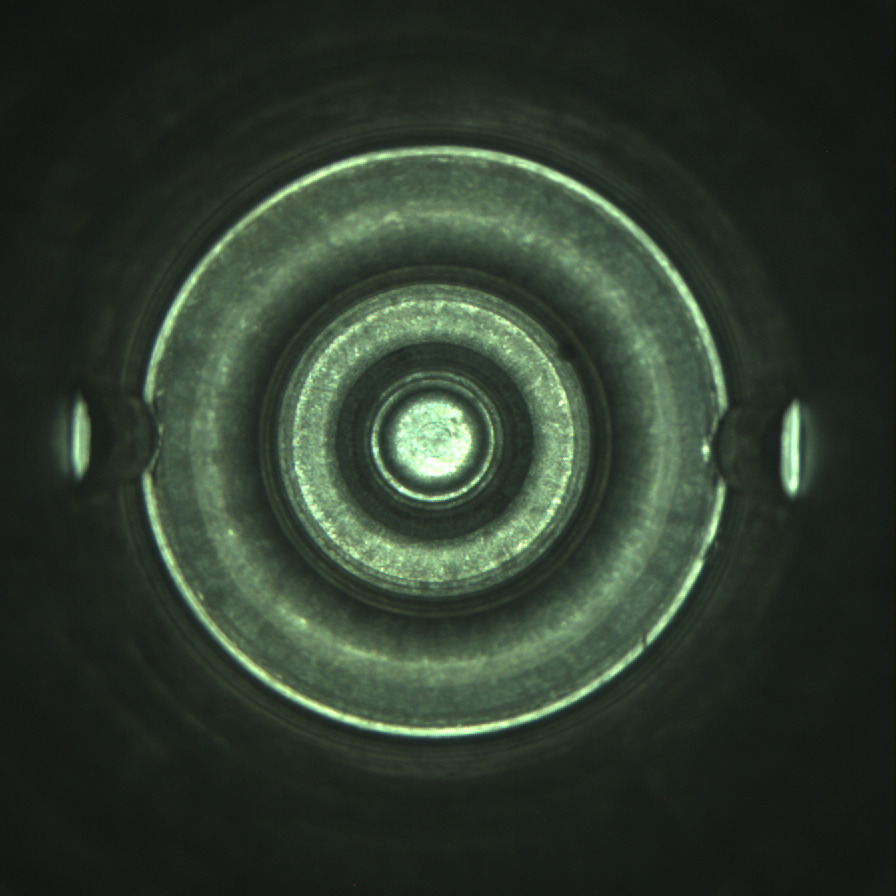
\includegraphics[width=\textwidth]{128___16740_0_0_1_OnLineAnalysis_0_hough_original}
      \caption{Immagine originale}
      \label{fig:p1_originale}
    \end{subfigure}
    \begin{subfigure}{.49\linewidth}
      \centering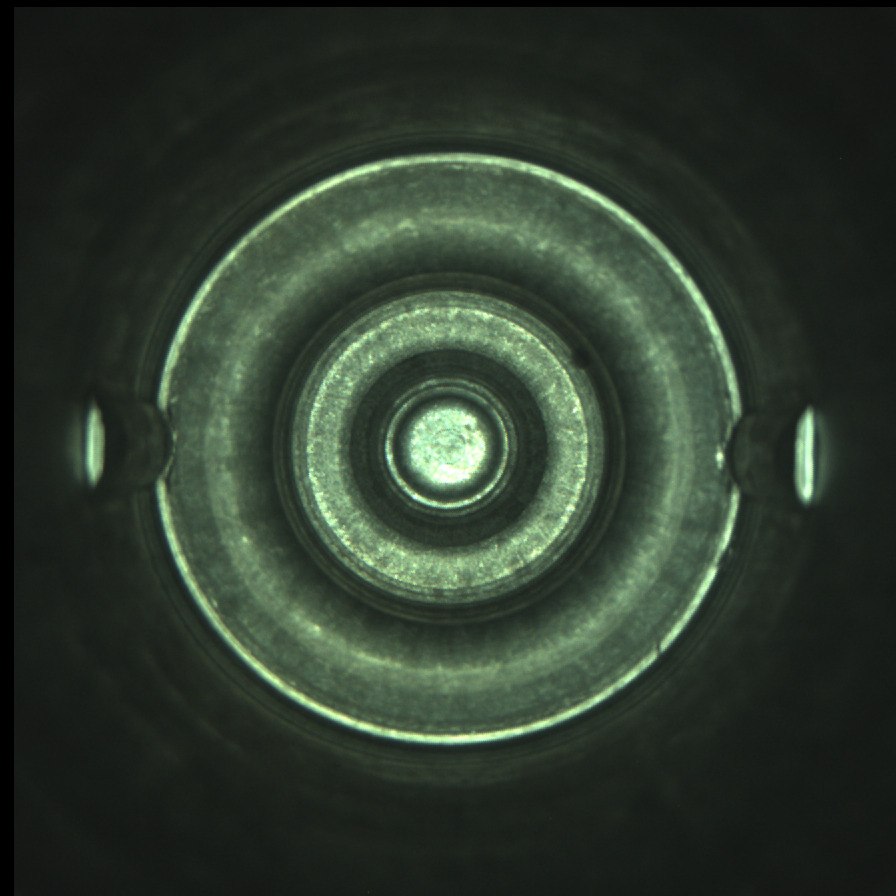
\includegraphics[width=\textwidth]{128___16740_0_0_1_OnLineAnalysis_0_hough}
      \caption{Immagine dopo il centramento}
      \label{fig:p1_centrata}
    \end{subfigure}
    \begin{subfigure}{.49\linewidth}
      \centering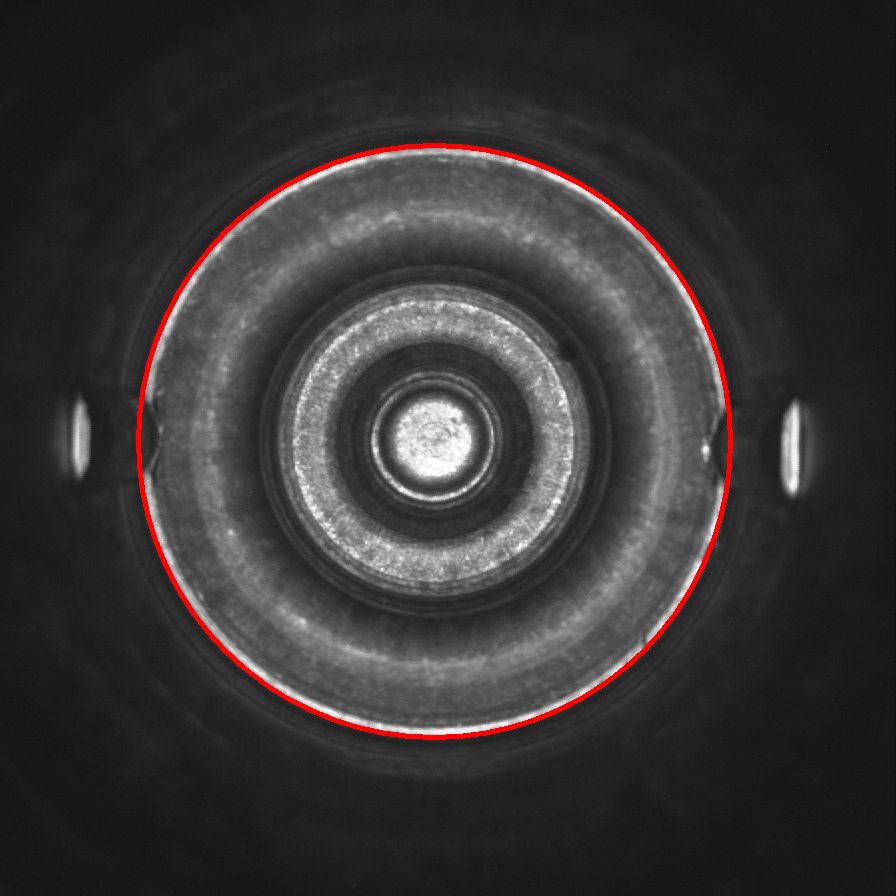
\includegraphics[width=\textwidth]{128___16740_0_0_1_OnLineAnalysis_0_hough_temp_pre_houghCirc}
      \caption{Circonferenza rilevata}
      \label{fig:p1_circ}
    \end{subfigure}
  \end{center}
  \caption{Esempio di centramento}
  \label{fig:centramento}
\end{figure}

\subsubsection{2 Equalizzazione}
Per gestire la variazione di luminosità tra immagini si utilizza \textit{histogram equalization}.
In questo modo le immagini in bianco e nero delle carcasse risultano molto più simili tra di loro e si vanno a mitigare i fastidiosi effetti di sovra illuminazione.

D'ora in poi verranno manipolate immagini in scala di grigi.
Questa scelta, validata dagli esperimenti, nasce principalmente considerando il fatto che le immagini sono in falsi colori.
Mantenendo il \textit{dataset} a colori manterremmo informazione che non ci è di alcuna utilità, ma soprattutto richiederemmo alla nostra rete neurale uno sforzo molto maggiore.
La rete, infatti, dovrebbe imparare a gestire, non solo le forme geometriche del pezzo, ma anche le sue colorazioni.

Nella figura~\ref{fig:equalizzazione} sono illustrate due carcasse conformi con luminosità differenti, affiancate dalla loro trasformazione.
% TODO mostrare l'immagine gray scale prima e dopo
\begin{figure}[ht] % TODO
  \begin{center}
    \begin{subfigure}{.49\linewidth}
      \centering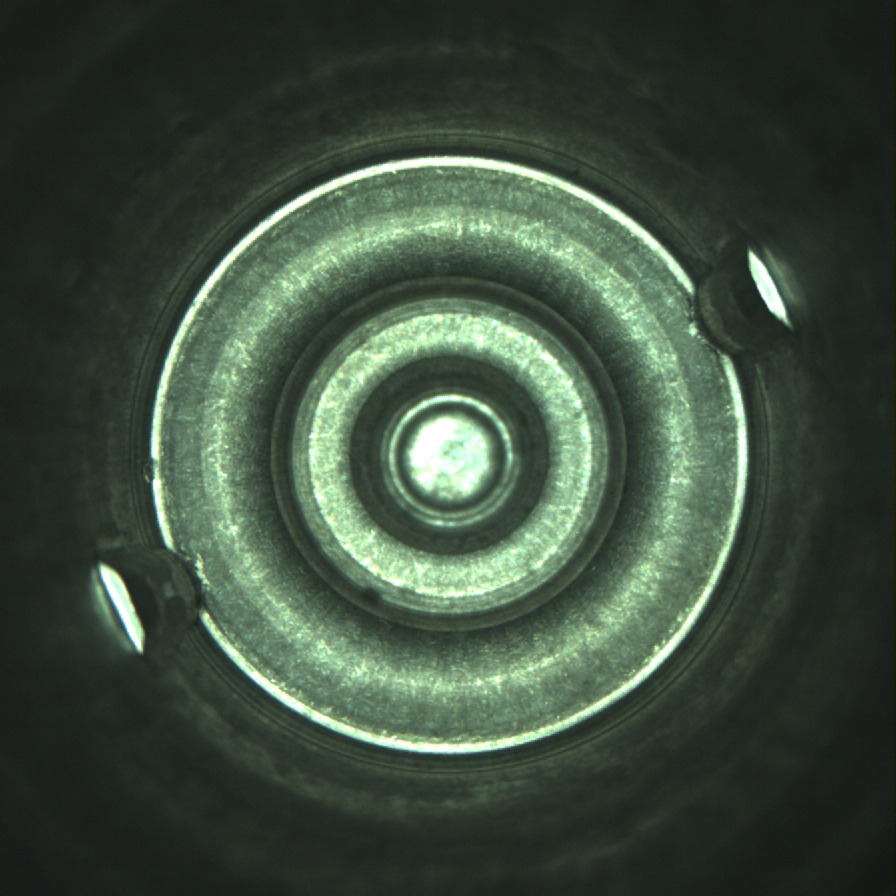
\includegraphics[width=\textwidth]{128___289_1_0_1_OnLineAnalysis}
      \caption{Immagine originale con alta luminosità}
      \label{fig:p2_originale_lum}
    \end{subfigure}
    \begin{subfigure}{.49\linewidth}
      \centering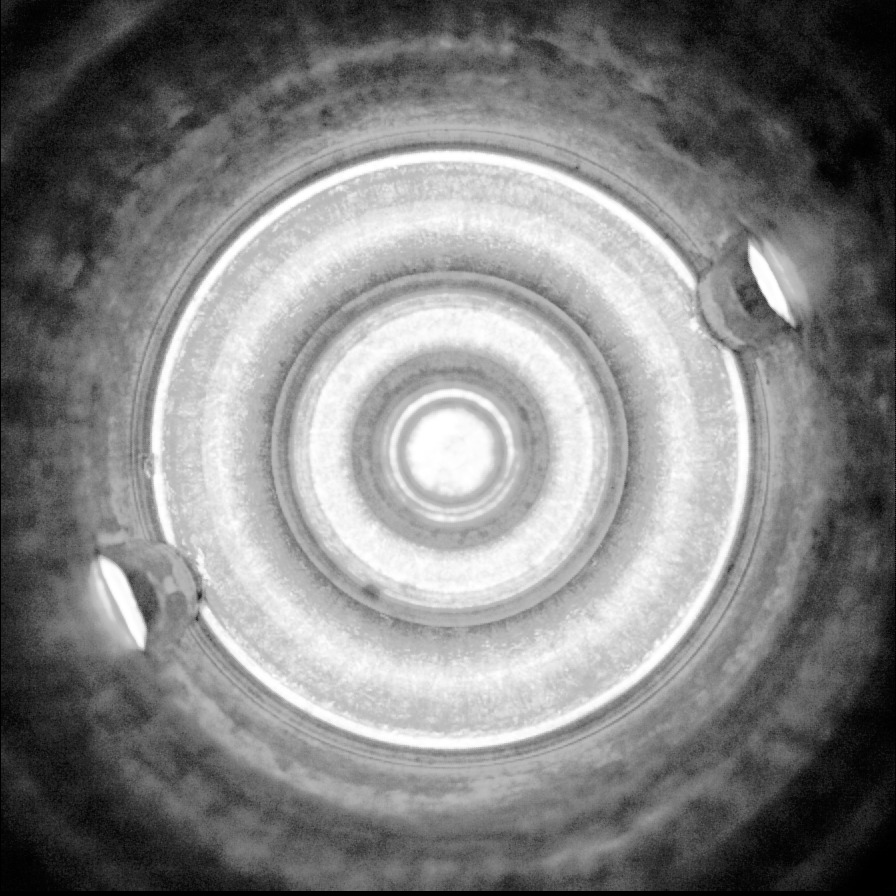
\includegraphics[width=\textwidth]{128___289_1_0_1_OnLineAnalysis_1_hist}
      \caption{Risultato dell'equalizzazione dell'immagine con alta luminosità}
      \label{fig:p2_equalizzata_lum}
    \end{subfigure}

    \begin{subfigure}{.49\linewidth}
      \centering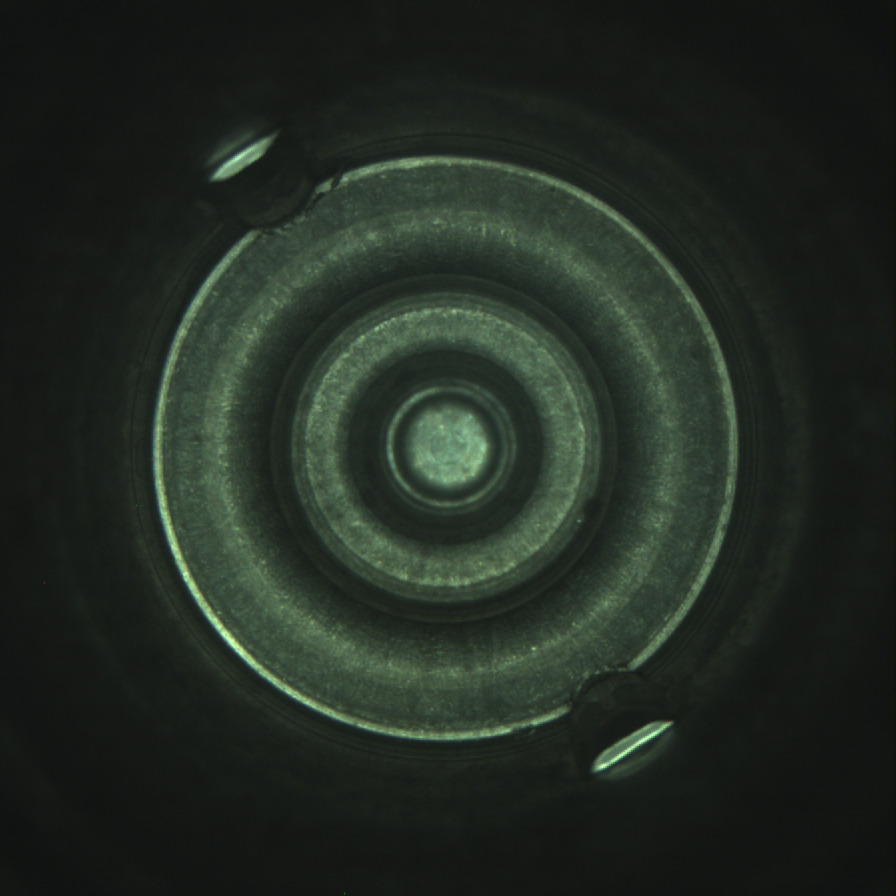
\includegraphics[width=\textwidth]{128___290_1_1_1_OnLineAnalysis}
      \caption{Immagine originale con bassa luminosità}
      \label{fig:p2_originale_scura}
    \end{subfigure}
    \begin{subfigure}{.49\linewidth}
      \centering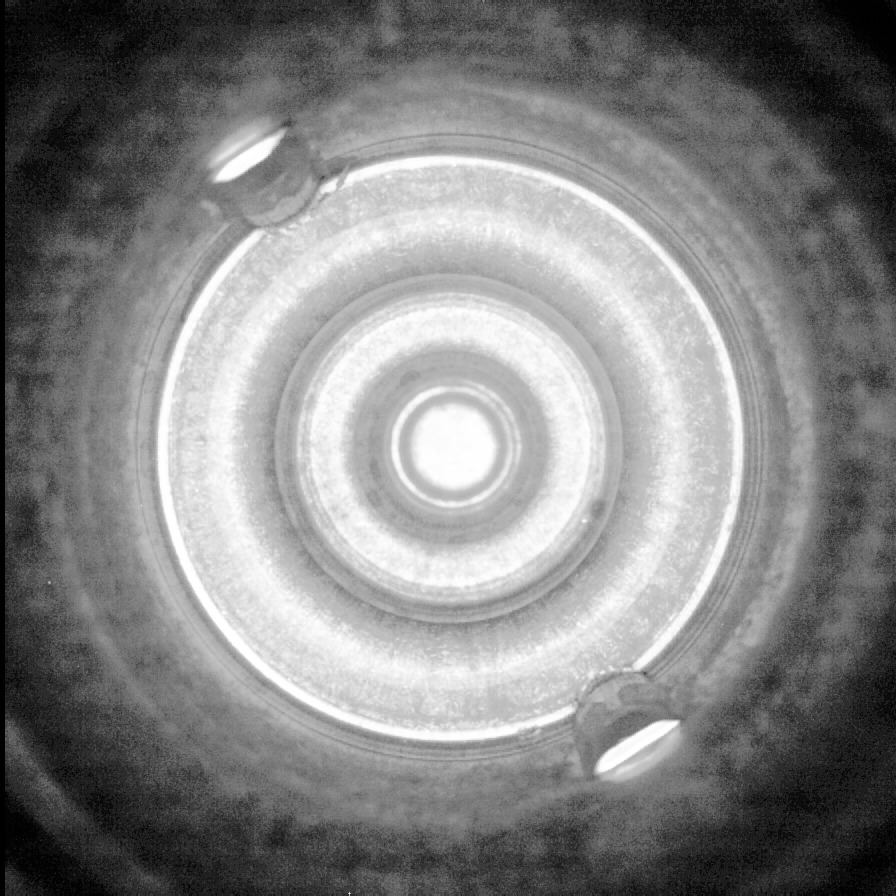
\includegraphics[width=\textwidth]{128___290_1_1_1_OnLineAnalysis_1_hist}
      \caption{Risultato dell'equalizzazione dell'immagine con bassa luminosità}
      \label{fig:p2_equalizzata_scura}
    \end{subfigure}

  \end{center}
  \caption{Esempio di equalizzazione}
  \label{fig:equalizzazione}
\end{figure}

\subsubsection{3 Smooth dell'immagine}
Utilizzando un filtro gaussiano è stato rimosso il rumore principale, ossia quello dovuto a graffi ed effetto ``sale e pepe''.
È stato fondamentale definire il filtro in modo che non fosse troppo aggressivo altrimenti si sarebbe rischiato di perdere anche l'informazione relativa alla colla.

In figura~\ref{fig:smooth} si mostra l'effetto dell'applicazione del kernel.
% TODO mostrare anche cosa succede se si esagera col filtro?
\begin{figure}[ht] % TODO
  \begin{center}
    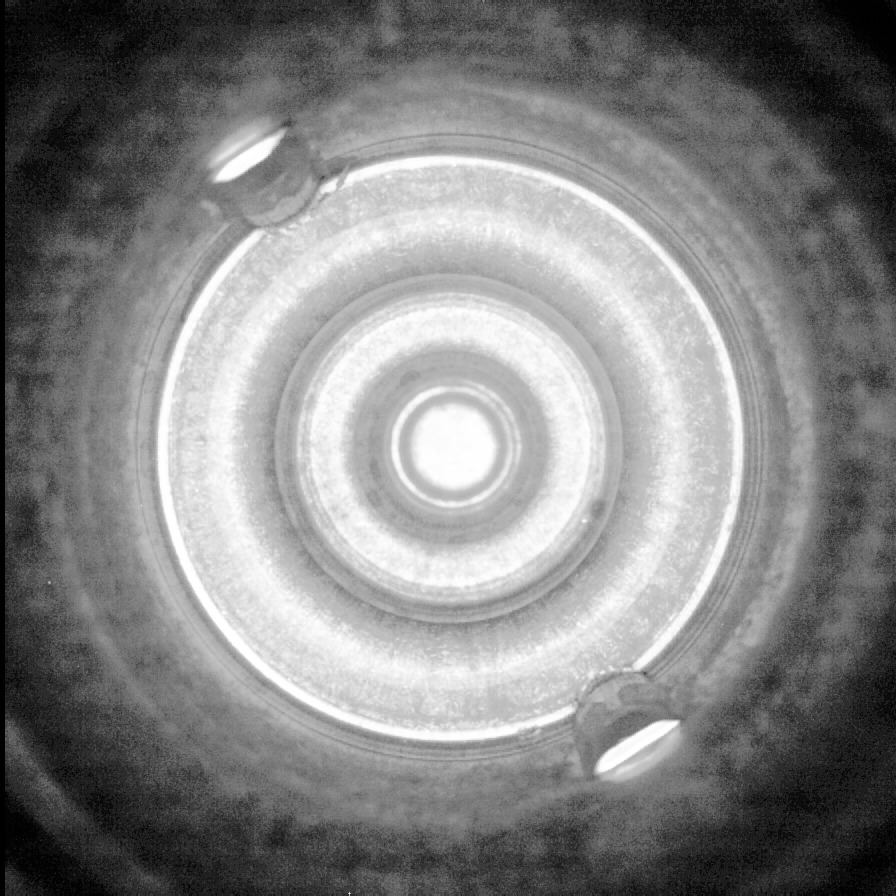
\includegraphics[width=0.49\textwidth]{128___290_1_1_1_OnLineAnalysis_1_hist}
    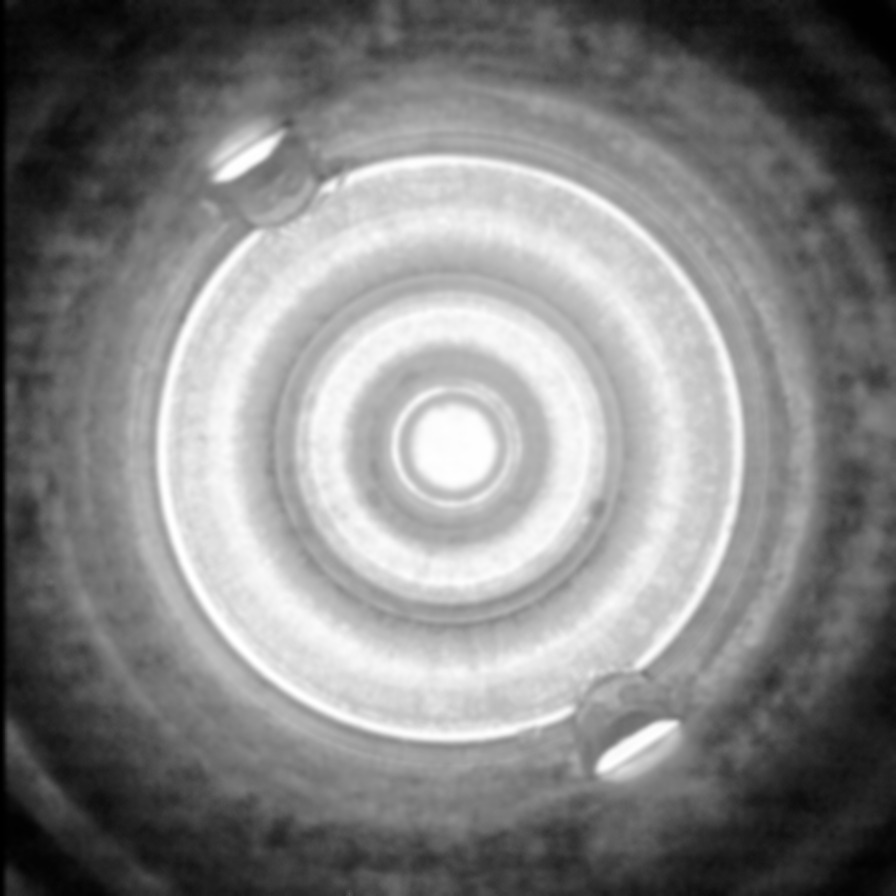
\includegraphics[width=0.49\textwidth]{128___290_1_1_1_OnLineAnalysis_2_bilFilt}
    \caption{Immagine prima e dopo l'applicazione del filtro di Gauss}
    \label{fig:smooth}
  \end{center}
\end{figure}

\subsubsection{4 Mascheramento}
L'area che nell'immagine corrisponde alla parete verticale della carcassa, ed in particolar modo alle due balze, deve essere rimossa.
Come abbiamo già sottolineato la posizione delle balze non è correlata con la presenza della colla.
Mentre si suppone che la colla non si presenti soltanto sulla parete verticale, ma che coli almeno fino a raggiungere il gradino più ampio.

Nella figura~\ref{fig:mask} è illustrato un conforme prima e dopo il mascheramento.

\begin{figure}[ht] % TODO
  \begin{center}
    \includegraphics[width=0.49\textwidth]{128___290_1_1_1_OnLineAnalysis_2_bilFilt}
    \includegraphics[width=0.49\textwidth]{128___290_1_1_1_OnLineAnalysis_3_mask}
    \caption{Immagine prima e dopo il mascheramento}
    \label{fig:mask}
  \end{center}
\end{figure}

\subsubsection{5 Crop}
A questo punto l'immagine contiene una grande porzione di pixel di colore nero, a causa del mascheramento.
Possiamo effettuare in operazione di \textit{crop} sapendo che il pezzo è centrato nell'immagine e conoscendo il raggio dell'area nera.
Osservando figura~\ref{fig:crop} ci si accorge che dopo il ritaglio l'immagine trasporta, in proporzione, molta più informazione.

\begin{figure}[ht] % TODO
  \begin{center}
    \includegraphics[width=0.5\textwidth]{128___290_1_1_1_OnLineAnalysis_3_mask}
    \includegraphics[width=0.35\textwidth]{128___290_1_1_1_OnLineAnalysis_4_crop}
    \caption{Immagine prima e dopo l'operazione di \textit{crop}}
    \label{fig:crop}
  \end{center}
\end{figure}

\subsubsection{6 Resizing}
Come ultima cosa viene effettuato un resizing dell'immagine.
Ogni elemento del dataset ha originariamente una dimensione di $896$x$896$ $pixel$, dopo le trasformazioni effettuate abbiamo un'immagine di dimensione circa $580$x$580px$.
Si ricorda che molte architetture di reti neurali accettano immagini di dimensione $224$x$224$.
È stato verificato se questa dimensione fosse accettabile anche nel caso di questo \textit{dataset)}: risulta che mantenere l'immagine ad una dimensione maggiore non comporta alcun vantaggio, mentre ridurla al di sotto dei $200$ $pixel$ di lato rende la classificazione difficile anche per un essere umano.

% $896$x$896$
% $580$x$580$
% $224$x$224$

\clearpage
\section {Data Augmentation}
Il \textit{Data Augmentation} è una tecnica che permette di aumentare le dimensioni del \textit{dataset}, generando nuovi elementi con caratteristiche verosimili.
Ciò risulta molto facile quando si manipolano immagini.
Queste possono essere facilmente traslate, ruotate o specchiate così da ottenere immagini differenti dall'originale, ma che contengono dell'informazione molto vicina a quello di partenza.
L'idea alla base della di queste trasformazioni è quella di incentivare la rete neurale a riconoscere gli oggetti a prescindere dalla loro orientazione.

Nel nostro caso si è deciso di ruotare i Conformi con angoli multipli di $45^\circ$.
Così facendo le macchioline ed i graffi compariranno in modo più uniforme, essendo distribuiti su più immagini.
Dopo questa operazione il numero di immagini Conformi a nostra disposizione è pari a $13752$, ossia $8$ immagini per ciascuno dei $1719$ campioni di partenza.

\subsection {Generazione Scarti Sintetici}
L'operazione di rotazione potrebbe essere applicata anche alle immagini Scarto, ma si è preferito optare per una manipolazione più complessa.

Sappiamo che le immagini degli Scarti sono state raccolte in un arco di tempo maggiore rispetto a quello dei Conformi.
Ciò può essere verificato confrontando alcune immagini delle due classi, prendiamo in esempio figura~\ref{fig:esempi_conformi} e figura~\ref{fig:esempi_scarti}, di pagine \pageref{fig:esempi_conformi} e \pageref{fig:esempi_scarti} rispettivamente.
Si può notare che alcuni Scarti presentano degli anelli di colore più scuro, come se la superficie fosse più sporca.
Questa caratteristica non compare in nessuna immagine della classe Conforme e sappiamo non essere in relazione con la presenza di colla.
Alcuni esemplari appartengono a lotti di carcasse molto più vecchi di quelli fotografati nei Conformi, per questo motivo si è cercato di ricreare degli Scarti che fossero più vicini ai pezzi recenti.
Si è prestata particolare attenzione a non generare immagini irreali, perché avrebbero invalidato qualsiasi tipo di risultato.
Infatti allenare un modello su un \textit{dataset} che non rispecchia la realtà renderebbe impossibile prevedere che il suo comportamento a livello applicativo.

In figura~\ref{fig:esempi_scarti_sintetici} è illustrato uno Scarto, il ritaglio della sua colla ed il risultato dell'applicazione di questa su due Conformi.
Innanzitutto tutte i tipi di colla sono stati ritagliati manualmente con un programma di manipolazione di immagini digitali.
Per ogni Scarto si è ottenuta un'immagine come quella riportata in figura~\ref{fig:ritaglio_colla}.
Notare come sia stato importante mantenere l'informazione riguardo la posizione della colla:
certe forme sono dovute al fatto che la colla è scivolata lungo i gradini del pezzo.
Si è preferito evitare di posizionare queste colle in zone prive di gradini o che avrebbero fatto si che la colla avesse altre conformazioni. % TODO ocio..

I ritagli appena creati non possono essere semplicemente applicati  sui conformi, basti pensare a come risulterebbe una colla fotografata in condizioni di grandi luminosità su una foto molto scura.
Per questo motivo la luminosità del ritaglio viene adattata a quello della zona che verrà coperta.
La figura~\ref{fig:scarto_sintetico_c} e la figura~\ref{fig:scarto_sintetico_d} mostrano come questo accorgimento dia risultati assolutamente verosimili: gli Scarti Sintetici sono stati ottenuti a partire da due Conformi distinti su cui è stata applicata la colla in figura~\ref{fig:ritaglio_colla}.
Per scrupolo è stato anche effettuato uno \textit{smooth} lungo il contorno della colla applicata, così da rendere più dolce la transizione tra il fondo della carcassa e il corpo della colla.
Si può dire che gli Scarti Sintetici siano indistinguibili dagli Scarti originali.



\begin{figure}[ht] % TODO
  \begin{center}
    \begin{tabular}{cc}
      \begin{subfigure}{.4\linewidth}
        \centering\includegraphics[width=\textwidth]{128___14097_1_0_1_OnLineAnalysis}
        \caption{Scarto}
      \end{subfigure} &

      \begin{subfigure}{.4\linewidth}
        \centering\includegraphics[width=\textwidth]{data_aug/colla_09}
        \caption{Colla ritagliata}
        \label{fig:ritaglio_colla}
      \end{subfigure} \\ \\

      \begin{subfigure}{.4\linewidth}
        \centering\includegraphics[width=\textwidth]{data_aug/128___372_1_1_1_OnLineAnalysis_colla_09}
        \caption{Scarto Sintetico}
        \label{fig:scarto_sintetico_c}
      \end{subfigure} &

      \begin{subfigure}{.4\linewidth}
        \centering\includegraphics[width=\textwidth]{data_aug/128___1283_1_0_1_OnLineAnalysis_colla_09}
        \caption{Scarto Sintetico}
        \label{fig:scarto_sintetico_d}
      \end{subfigure}
    \end{tabular}
    \caption{Scarto e Scarti Sintetici a confronto}
    \label{fig:esempi_scarti_sintetici}
  \end{center}
\end{figure}






























% TODO in caso sarebe un Chapter a sé
%\section {La strada proposta}
% Simile a quanto detto in considerazioni_pixelwise_diff
%Mostrare qual'è l'obbiettivo che si vuole raggiungere con gli AE
%Spiegare che sono elastici e facili da allenare
%Il dataset non richiede dispendioso labeling
